%%% The main file. It contains definitions of basic parameters and includes all other parts.

%% Settings for single-side (simplex) printing
% Margins: left 40mm, right 25mm, top and bottom 25mm
% (but beware, LaTeX adds 1in implicitly)
\documentclass[12pt,a4paper]{report}
\setlength\textwidth{145mm}
\setlength\textheight{247mm}
\setlength\oddsidemargin{15mm}
\setlength\evensidemargin{15mm}
\setlength\topmargin{0mm}
\setlength\headsep{0mm}
\setlength\headheight{0mm}
% \openright makes the following text appear on a right-hand page
\let\openright=\clearpage
\usepackage{xcolor, soul}

%% Settings for two-sided (duplex) printing
% \documentclass[12pt,a4paper,twoside,openright]{report}
% \setlength\textwidth{145mm}
% \setlength\textheight{247mm}
% \setlength\oddsidemargin{14.2mm}
% \setlength\evensidemargin{0mm}
% \setlength\topmargin{0mm}
% \setlength\headsep{0mm}
% \setlength\headheight{0mm}
% \let\openright=\cleardoublepage


%% Generate PDF/A-2u
\usepackage[a-2u]{pdfx}

%% Character encoding: usually latin2, cp1250 or utf8:
\usepackage[utf8]{inputenc}

%% Prefer Latin Modern fonts
\usepackage{lmodern}

%% Further useful packages (included in most LaTeX distributions)
\usepackage{amsmath}        % extensions for typesetting of math
\usepackage{amsfonts}       % math fonts
\usepackage{amsthm}         % theorems, definitions, etc.
\usepackage{bbding}         % various symbols (squares, asterisks, scissors, ...)
\usepackage{bm}             % boldface symbols (\bm)
\usepackage{graphicx}       % embedding of pictures
\usepackage{fancyvrb}       % improved verbatim environment
\usepackage[round]{natbib}         % citation style AUTHOR (YEAR), or AUTHOR [NUMBER]
\usepackage[nottoc]{tocbibind} % makes sure that bibliography and the lists
			    % of figures/tables are included in the table
			    % of contents
\usepackage{dcolumn}        % improved alignment of table columns
\usepackage{booktabs}       % improved horizontal lines in tables
\usepackage{paralist}       % improved enumerate and itemize
%TODO: toto neni potreba? zpusobovalo error message...
%\usepackage[usenames]{xcolor}  % typesetting in color
\usepackage{algorithm}
\usepackage[noend]{algpseudocode}

\usepackage{bbm}
\usepackage{mathtools}
\usepackage{siunitx}
\usepackage{import}
\usepackage{varwidth}% http://ctan.org/pkg/varwidth
\usepackage{subcaption}

%%% Basic information on the thesis

% Thesis title in English (exactly as in the formal assignment)
\def\ThesisTitle{Decoding visual stimuli from cortical activity}

% Author of the thesis
\def\ThesisAuthor{Vojtěch Vašek}
\def\ThesisAuthorTitle{Mgr. Vojtěch Vašek}

% Year when the thesis is submitted
\def\YearSubmitted{2023}

% Name of the department or institute, where the work was officially assigned
% (according to the Organizational Structure of MFF UK in English,
% or a full name of a department outside MFF)
\def\Department{Department of Cell Biology}

% Is it a department (katedra), or an institute (ústav)?
\def\DeptType{Department}

% Thesis supervisor: name, surname and titles
\def\Supervisor{Mgr. Ján Antolík, Ph.D.}
\def\Consultant{Luca Baroni, M.Sc.}

% Supervisor's department (again according to Organizational structure of MFF)
\def\SupervisorsDepartment{Department of Software and Computer Science Education} % FIXME

% Study programme and specialization
\def\StudyProgramme{Bachelor in Bioinformatics}
\def\StudyBranch{Bioinformatics}

% An optional dedication: you can thank whomever you wish (your supervisor,
% consultant, a person who lent the software, etc.)
\def\Dedication{%
I would like to dedicate this thesis to my loving wife, whose patience and support have been my pillar of strength. Her belief in me and the constant smile of our daughter have brought immense joy and motivation.

I also want to express my gratitude to my supervisor, Mgr. Ján Antolík, Ph.D., and also my consultant Luca Baroni, M.Sc., their invaluable wisdom, expertise, ideas, and insights have significantly contributed to shaping this thesis. Their guidance and encouragement have helped me achieve the goals of this thesis.
}

% Abstract (recommended length around 80-200 words; this is not a copy of your thesis assignment!)

\def\Abstract{%
This thesis aims to develop a machine learning model that can decode stimulus images from cortical activity in the primary visual cortex (V1) to understand the relationship between V1 activity and visual perception. The limited availability of biological data makes it necessary to use the spiking neural network model of V1 to generate the underlying training data. Machine learning techniques, particularly neural networks, will be explored to generate high-quality stimulus images. Standard loss functions, as well as discriminator loss from GAN networks training, will be used to train the decoding models. Linear regression models will be used baseline. The research questions to be addressed include the best decoding approach, the impact of the number of neurons recorded or stimuli presented, the loss of information in high frequencies domain and the effect of intrinsic noise in neural responses on reconstructing visual stimuli. This thesis proposes a trainable convolutional network, which outperforms other baseline models such as linear regression. We observe that the loss function producing the best results is the MSSSIM. However, the intrinsic noise in neural responses limits the reconstruction, and only low frequencies are being reconstructed. The size of the dataset and the number of cortical neurons, specifically inhibitory neurons from layer L4 are important for the decoding. This research may have implications for the development of visual prosthetics and virtual reality systems.
}

% 3 to 5 keywords (recommended), each enclosed in curly braces
\def\Keywords{%
{computational neuroscience}, {deep learning}, {spiking neural networks}
}

%% The hyperref package for clickable links in PDF and also for storing
%% metadata to PDF (including the table of contents).
%% Most settings are pre-set by the pdfx package.
\hypersetup{unicode}
\hypersetup{breaklinks=true}

% Definitions of macros (see description inside)
%%% This file contains definitions of various useful macros and environments %%%
%%% Please add more macros here instead of cluttering other files with them. %%%

%%% Minor tweaks of style

% These macros employ a little dirty trick to convince LaTeX to typeset
% chapter headings sanely, without lots of empty space above them.
% Feel free to ignore.
\makeatletter
\def\@makechapterhead#1{
  {\parindent \z@ \raggedright \normalfont
   \Huge\bfseries \thechapter. #1
   \par\nobreak
   \vskip 20\p@
}}
\def\@makeschapterhead#1{
  {\parindent \z@ \raggedright \normalfont
   \Huge\bfseries #1
   \par\nobreak
   \vskip 20\p@
}}
\makeatother

% This macro defines a chapter, which is not numbered, but is included
% in the table of contents.
\def\chapwithtoc#1{
\chapter*{#1}
\addcontentsline{toc}{chapter}{#1}
}

% Draw black "slugs" whenever a line overflows, so that we can spot it easily.
\overfullrule=1mm

%%% Macros for definitions, theorems, claims, examples, ... (requires amsthm package)

\theoremstyle{plain}
\newtheorem{thm}{Theorem}
\newtheorem{lemma}[thm]{Lemma}
\newtheorem{claim}[thm]{Claim}

\theoremstyle{plain}
\newtheorem{defn}{Definition}

\theoremstyle{remark}
\newtheorem*{cor}{Corollary}
\newtheorem*{rem}{Remark}
\newtheorem*{example}{Example}

%%% An environment for proofs

%%% FIXME %%% \newenvironment{proof}{
%%% FIXME %%%   \par\medskip\noindent
%%% FIXME %%%   \textit{Proof}.
%%% FIXME %%% }{
%%% FIXME %%% \newline
%%% FIXME %%% \rightline{$\square$}  % or \SquareCastShadowBottomRight from bbding package
%%% FIXME %%% }

%%% An environment for typesetting of program code and input/output
%%% of programs. (Requires the fancyvrb package -- fancy verbatim.)

%%% KAPPA macros for unification of "special" words/sentences
\newcommand{\term}[1]{\textit{#1}}
\newcommand{\zvyr}[1]{\textbf{#1}}
\newcommand{\todo}[1]{}
\renewcommand{\todo}[1]{{\color{red} TODO: {#1}}}
\newcommand{\remark}[1]{{\color{red} VF: {#1}}}
\newcommand{\note}[2]{{\color{red} NOTE[{#1}]: {#2}}}

%-- MMMakro ------------------                                                  
\def\##1{\relax\ifmmode\mathchoice      % italic bold vector, e.g. $\#{x}$
{\mbox{\boldmath$\displaystyle#1$}}
{\mbox{\boldmath$\textstyle#1$}}
{\mbox{\boldmath$\scriptstyle#1$}}
{\mbox{\boldmath$\scriptscriptstyle#1$}}\else
\hbox{\boldmath$\textstyle#1$}\fi}
\def\m#1{\mathbf{#1}}                  % bold matrix, e.g. $\m{A}$

\newcommand{\SC}{{\cal C}}
\newcommand{\SL}{{\cal L}}
\newcommand{\SX}{{\cal X}}
\newcommand{\SY}{{\cal Y}}
\newcommand{\SD}{{\cal D}}
\newcommand{\SH}{{\cal H}}
\newcommand{\SG}{{\cal G}}

\DeclareMathOperator*{\argmax}{arg\,max}
\DeclareMathOperator*{\argmin}{arg\,min}
\DeclarePairedDelimiter{\ceil}{\lceil}{\rceil}

\DefineVerbatimEnvironment{code}{Verbatim}{fontsize=\small, frame=single}

%%% The field of all real and natural numbers
\newcommand{\R}{\mathbb{R}}
\newcommand{\N}{\mathbb{N}}

%%% Useful operators for statistics and probability
\DeclareMathOperator{\pr}{\textsf{P}}
\DeclareMathOperator{\E}{\textsf{E}\,}
\DeclareMathOperator{\var}{\textrm{var}}
\DeclareMathOperator{\sd}{\textrm{sd}}

%%% Transposition of a vector/matrix
\newcommand{\T}[1]{#1^\top}

%%% Various math goodies
\newcommand{\goto}{\rightarrow}
\newcommand{\gotop}{\stackrel{P}{\longrightarrow}}
\newcommand{\maon}[1]{o(n^{#1})}
\newcommand{\abs}[1]{\left|{#1}\right|}
\newcommand{\dint}{\int_0^\tau\!\!\int_0^\tau}
\newcommand{\isqr}[1]{\frac{1}{\sqrt{#1}}}

%%% Various table goodies
\newcommand{\pulrad}[1]{\raisebox{1.5ex}[0pt]{#1}}
\newcommand{\mc}[1]{\multicolumn{1}{c}{#1}}


% Title page and various mandatory informational pages
\begin{document}
%%% Title page of the thesis and other mandatory pages

%%% Title page of the thesis

\pagestyle{empty}
\hypersetup{pageanchor=false}
\begin{center}

% TODO: other thesis on this faculty don't use logo...
%\centerline{\mbox{\includegraphics[width=166mm]{./img/logo-en.pdf}}}

\vspace{-8mm}
\vfill

{\bf\Large BACHELOR THESIS}

\vfill

{\LARGE\ThesisAuthor}

\vspace{15mm}

{\LARGE\bfseries\ThesisTitle}

\vfill

\Department

\vfill

\begin{tabular}{rl}

Supervisor of the bachelor thesis: & \Supervisor \\
\noalign{\vspace{2mm}}
Consultant of the bachelor thesis: & \Consultant \\
\noalign{\vspace{2mm}}
Study programme: & \StudyProgramme \\
\noalign{\vspace{2mm}}
Study branch: & \StudyBranch \\
\end{tabular}

\vfill

Prague \YearSubmitted

\end{center}

\newpage

%%% Here should be a bound sheet included -- a signed copy of the "master
%%% thesis assignment". This assignment is NOT a part of the electronic
%%% version of the thesis. DO NOT SCAN.

%%% A page with a solemn declaration to the master thesis

\openright
\hypersetup{pageanchor=true}
\pagestyle{plain}
\pagenumbering{roman}
\vglue 0pt plus 1fill

\noindent
I declare that I carried out this bachelor thesis independently, and only with the cited
sources, literature and other professional sources.

\medskip\noindent
I understand that my work relates to the rights and obligations under the Act No.~121/2000 Sb.,
the Copyright Act, as amended, in particular the fact that the Charles
University has the right to conclude a license agreement on the use of this
work as a school work pursuant to Section 60 subsection 1 of the Copyright Act.

\vspace{10mm}

\hbox{\hbox to 0.5\hsize{%
In Prague date 3. 5. 2023
\hss}\hbox to 0.5\hsize{%
% TODO: signature
\hss}}

\vspace{20mm}
\newpage

%%% Dedication

\openright

\noindent
\Dedication

\newpage

%%% Mandatory information page of the thesis

\openright

\vbox to 0.5\vsize{
\setlength\parindent{0mm}
\setlength\parskip{5mm}

Title:
\ThesisTitle

Author:
\ThesisAuthorTitle

\DeptType:
\Department

Supervisor:
\Supervisor, \SupervisorsDepartment

Consultant:
\Consultant, \SupervisorsDepartment

Abstract:
\Abstract

Keywords:
\Keywords

\vss}

\newpage

\openright
\pagestyle{plain}
\pagenumbering{arabic}
\setcounter{page}{1}


%%% A page with automatically generated table of contents of the master thesis

\tableofcontents

%%% Each chapter is kept in a separate file
% ==================================================
% ==================================================
\chapter{Introduction}
\label{intro}
The cerebral visual system is a complex biological system that has been a subject of research for almost a century. The primary animal models to study visual cortex are macaques~\citep{felleman1991distributed, boussaoud1990pathways}, cat, ferret, and  mouse~\citep{marshel2011functional, beltramo2019collicular}, but human studies are also common~\citep{boynton1996linear, wandell2007visual}. The primary visual cortex (V1) is the first cortical stage of visual processing, responsible for receiving and processing visual information from the retina. The cortical activity generated by V1 neurons can provide insights into visual perception.

Recent advancements in spiking neural network models have enabled us to simulate the activity of neurons in V1 in response to visual stimuli~\citep{antolik2018comprehensive}. By generating V1 cortical activity patterns through these models, we can study how the visual system processes and interprets visual stimuli, and how this activity relates to the perception of the individual.

One potential application of these models is to develop visual prostheses for individuals with visual impairments, such as blindness. By using V1 cortical activity generated by a spiking neural network, we can potentially design stimulation protocols for the visual prosthetic system, to restore some degree of vision to these individuals by generating visual stimuli that mimic the activity in their visual cortex.

However, before we can proceed with such clinical applications we need to first understand the relationship between the cortical activity in V1 and visual perception, which is the goal of this thesis. Specifically, we aim to develop a model that can decode stimulus images from the cortical activity in V1. This will enable us to explore the relationship between V1 activity and visual perception and develop new insights into how the visual system processes and interprets visual information.

One of the challenges of developing a model that can decode stimulus images from cortical activity is the limited availability of biological data. Collecting a sufficient amount of biological data is not only time-consuming but also requires extensive resources and expertise. Therefore, it makes sense to use the spiking neural network model of the V1, developed by Antolík and colleagues~\citep{antolik2018comprehensive}, which can potentially generate an unlimited amount of data needed to train these models. After this step, the models could be evaluated on expensive real biological data.

We will explore the use of machine learning techniques, particularly neural networks, to generate stimulus images from the V1 cortical activity model. Neural networks have been extensively used in computer vision and image processing, and they have shown great potential for generating high-quality images. One of the most common approaches is to use convolutional neural networks (CNNs) for image generation, as they are capable of capturing complex image features and patterns~\citep{radford2015unsupervised, xu2018attngan}.

To train our decoding models, we will use standard loss functions such as L1, MSE, SSIM, or MSSSIM, as well as more advanced discriminator loss from GAN networks training~\citep{goodfellow2014generative, goodfellow2020generative}. We will also employ linear regression models to examine the relationship between the V1 cortical activity and the corresponding stimulus images. This approach has been successfully used in previous studies to decode visual information from cortical activity~\citep{kay2008identifying}.

%The objective of this research is to develop a method for generating high-quality stimulus images based on cortical activity by combining the V1 cortical activity model with machine learning techniques. The spiking model of V1 proposed by~\citep{antolik2018comprehensive} is utilized to generate the dataset for training our models. The integration of machine learning techniques with the V1 cortical activity model is expected to result in a more accurate and efficient method for reconstructing visual stimuli.

\subsection*{Prior work}

In this thesis, we review several approaches for decoding visual information from neural activity. Retinal ganglion cell spikes have been used as a decoding tool by many researchers, including~\citep{zhang2020reconstruction}. We utilize their model as our second baseline along with the linear regression, which is a linear decoder, that is proposed by a few other following papers~\citep{Parthasarathy153759, kay2008identifying, kim2021nonlinear}.
Similar to the previous, in this paper~\citep{Parthasarathy153759}, they employed a linear decoder in their study and improved image reconstruction using a CNN encoder-decoder architecture.
This paper~\citep{kay2008identifying}, used human brain activity from visual areas V1, V2, and V3 as measured by fMRI. They employed linear decoders for decoding the information.
Another approach, as proposed~\citep{qiao2020biggan}, used GANs to decode images. The GAN is provided with Gaussian noise and a category of the image, which is classified by a model based on fMRI brain activity. The generated image is then encoded back to the activity vector by another model and the predicted and true activity vectors are evaluated by an evaluator model. They use fMRI data from the human's brain visual areas V1, V2, V3, and V4. This approach is not suitable, as the categories of images are unknown and the data we use are not fMRI.
Authors of~\citep{kim2021nonlinear} proposed a novel method for decoding visual information from retinal ganglion cells. They used a combination of linear and neural network-based decoders, and a deblurring network to improve the image reconstruction.

Despite the fact, that many researchers study this field, the neural decoding problem remains a significant open challenge. The reason is that the current methods still give poor results in terms of resolving high-frequencies, which describe the fine details in images.

In this thesis, specifically, we aim to mainly address the following questions:

\begin{itemize}
    \item What is the best decoding approach in terms of choice of architecture, and loss function to reconstruct stimuli from the neural activity?
    \item How does the number of neurons recorded or the number of stimuli presented affect results?
    \item Does the intrinsic noise in neural responses represent a substantial limitation to reconstructing visual stimuli?
    \item Besides these questions, we also want to evaluate the influence of different image perturbations on the behavior of different loss functions. 
\end{itemize}


\subsection*{Outline}

In summary, our main focus is to decode the cortical activity and generate stimulus images that accurately represent the visual information processed by the brain. The development of a reliable and accurate model for stimulus image generation has the potential to offer new insights into the visual system and its processing of visual information. By shedding light on the cortical activity in V1 and its role in visual perception, this research may have implications for the development of visual prosthetics, brain-machine interfaces, and virtual reality systems. 
To achieve the stated goals, we utilize the spiking neural model of the V1 cortex developed by Antolik and colleagues~\cite{antolik2018comprehensive}. This model enables us to address questions that would otherwise be hard to answer, such as the impact of the number of neurons and samples in the dataset. Experimental recordings of such large volumes of biological data would be nearly impossible.


The following is the structure of the thesis. Chapter~\ref{methods} describes the proposed models as well as baseline models, loss functions for decoding the stimuli image, and the implementation details. Chapter~\ref{dataset} is dedicated to the description of the datasets we use for training and testing our models. Chapter~\ref{experiments} contains experimental evaluations of the models, and loss functions, but also experiments on the cortical neurons. The final Chapter~\ref{conclusion} comprises of concluding remarks and recommendations for possible future work.
%% ==================================================
% ==================================================
\chapter{State of the Art}
\label{sota}

% ==================================================
% ==================================================
\chapter{Methods}
\label{methods}
This chapter describes the methods used in our experiments. In section~\ref{methods:models}, we start by defining the problem~\ref{methods:models:problem-definition}, then we present one simple approach to decode images using linear regression and four more advanced ones which use neural networks, some of which are inspired by~\citep{zhang2020reconstruction}. We use the model from this paper, along with the linear regression, as a baseline comparison.

In the following section~\ref{methods:losses}, we present several loss functions that we use for training and testing the model performance. We use simple ones like $L_1$ ~\ref{methods:losses:L1} or MSE ~\ref{methods:losses:MSE}, as well as a more complex one implemented through the use of another neural network ~\ref{methods:losses:adversarial}.

The details about the software and packages we used are in the last section~\ref{methods:implementation-details}.

The experiments using these models and these losses are described in the subsequent chapter~\ref{experiments}.

% ==================================================
\section{Models}
\label{methods:models}
To address the problem of decoding visual stimuli, we implemented several different models. Some were selected as a simple baseline~\ref{methods:models:linear-regression}, and others were based on state-of-the-art CNN networks~\ref{methods:models:CNNv4} for image decoding~\citep{zhang2020reconstruction}. The ones that performed the best are presented in this section. We start this section by properly defining the problem we are solving~\ref{methods:models:problem-definition}.


% **************************************************
\subsection{Problem Definition}
\label{methods:models:problem-definition}
The problem of decoding image stimuli from cortical activity in this thesis is defined as follows. The cortical activity consists of the responses of the neurons in the primary visual cortex to visual stimuli. The goal of the decoding process is to accurately generate a visual stimulus image that is similar to the one presented to the subject based on the recorded cortical activity.

Let us assume that we are provided with a cortical activity encoded as $\#{x} \in \SX$ where $\SX = \mathbb{R}^{n}$ denotes the space of all possible cortical activity encodings using $n$ neurons.
We are trying to predict stimuli $\#{s} \in \SY$, where $\SY = [0;1]^{h \times w}$ denotes space of all possible stimuli images of width $w$ and height $h$. The stimuli images are therefore grayscale and the pixel values are in the range [0;1], where 0 is the darkest and 1 is the lightest value. In our settings, we can assume $w=h$.

The goal is to create a generator $g:\ \SX \rightarrow \SY$ from a space of all such functions $\SG$ which for given cortical activity vector $\#{x} \in \SX$ predicts a decoded stimulus image $\#{s} \in \SY$. Let us first define
\begin{equation}
\label{equation:predictor-loss}
l(\#{s}, g, \#{x}) = \SL(\#{s}, g(\#{x} ; \#\theta))\:,
\end{equation}
% \begin{equation}
% \label{equation:predictor-loss-mean}
% \SL(\#{s}, g(\#{x} ; \#\theta)) = \sum_{i=1, j=1}^{w, h}{\SL_{i,j}(s_{i,j}, g_{i,j}(\#{x} ; \#\theta))} \cdot \frac{1}{w+h}\:,
% \end{equation}
% where $\SL(\#{s}, g(\#{x} ; \#\theta))$ resp. $\SL_{i,j}(s_{i,j})$ is an arbitrary differentiable loss function (image-wise resp. point-wise defined) (find more details about used loss functions in section~\ref{methods:losses}) which given the stimulus $\#{s} \in \SY$ and generated image given by the generator function $g$ returns the loss value. Values $\#\theta$ are the parameters of the generator function. By $f_{i,j}$ we denote pixel value on $i$-th column and $j$-th row of function $f$.

% Due to minimization, we can simplify the formula~\ref{equation:predictor-loss-mean}, we can also omit the parameters of function $g$ for brevity
% \begin{equation}
% \label{equation:simplified-loss}
% \SL(\#{s}, g) = \sum_{i=1, j=1}^{w, h}{\SL_{i,j}(s_{i,j}, g_{i,j})}\:.
% \end{equation}
where $\SL(\#{s}, g(\#{x} ; \#\theta))$ is an arbitrary differentiable loss function (find more details about used loss functions in section~\ref{methods:losses}). Values $\#\theta$ are the parameters of the generator function.


We want such $g \in \SG$, lets denote it $g^* \in \SG$, that minimizes the value $l(\#{s},g,\#{x})$:

\begin{equation}
%\label{equation:predictor}
% l_{min}(\#{x}) = \argmin_{\#{s}\in \SY, g\in \SG}{l(\#{s},g,\#{x})}\:,
\argmin_{\#{s}\in \SY}l(\#{s},g^*,\#{x}) = \argmin_{\#{s}\in \SY, g\in \SG}{l(\#{s},g,\#{x})}\:.
\end{equation}
%  $g^*$ satisfies
% \begin{equation}
% %\label{equation:predictor-loss-mean}
% \argmin_{\#{s}\in \SY}l(\#{s},g^*,\#{x}) = l_{min}(\#{x})\:.
% \end{equation}


We present several CNN models in the following sections to find $g^*$ using only the standard CNN layers -- namely convolutional layers, fully connected layers, convolutional transpose layers, and batch normalization layers. The CNN models use standard ReLU activation function internally and utilize a sigmoid activation function in the final layer, resulting in the output values being constrained within the range of [0, 1], which matches the range of the stimuli images.

We learn the model parameters, and therefore train the model to approximate $g^*$, by minimizing the formula
\begin{equation}
\label{equation:predictor-loss-minimization}
L(\#\theta) = \sum_{j=1}^m{\SL(\#{s}, g(\#{x} ; \#{\theta}))}\:,
\end{equation}
where $\{(\#{x}^j, \#{s}^j) \in (\SX \times \SY) \mid j=1,2,\dots,m\}$ is the training dataset with $m$ training samples.


% **************************************************
\subsection{Linear Regression}
\label{methods:models:linear-regression}
As a simple baseline, linear regression was used based on its deterministic properties to always converge to the same optimum value. The goal of linear regression is to find a linear relationship that best fits the given data.

In simple linear regression, the relationship between the dependent variable Y and the independent variable X is modeled as a straight line. The equation of the line can be written as:

\begin{equation}
Y = \beta_0 + \beta_1 X + \epsilon
\end{equation}

where $\beta_0$ is the intercept, $\beta_1$ is the slope, and $\epsilon$ is the error term which represents the unexplained variability in the data.

The objective of linear regression is to estimate the values of the parameters $\beta_0$ and $\beta_1$ that best fit the data. This is typically done using the method of least squares, which involves minimizing the sum of the squared errors:

\begin{equation}
\sum_{i=1}^{n}(Y_i - \beta_0 - \beta_1 X_i)^2
\end{equation}

where $n$ is the number of observations.

In our case, to be able to use this method, we linearize the stimuli images $\#{s} \in \SY$ from 2D matrices $w \times h$ to vectors of size $w * h$.


% **************************************************
\subsection{CNNv1}
\label{methods:models:CNNv1}
The first neural network presented is a CNN model that generates an image on the latest layer. 

It has a sequential architecture with several transposed convolutional layers with increasing numbers of filters. Each transposed convolutional layer is followed by a batch normalization layer and a ReLU activation function. The final layer is a transposed convolutional layer with a sigmoid activation function that outputs the reconstructed image.

The network has a total of 278,197,825 parameters, all of which are trainable. The architecture is graphically presented on the picture~\ref{img:methods:models:CNNv1}. Since the output is not 110x110px, we use bilinear interpolation to create the proper output size.

\begin{figure}[H]\centering
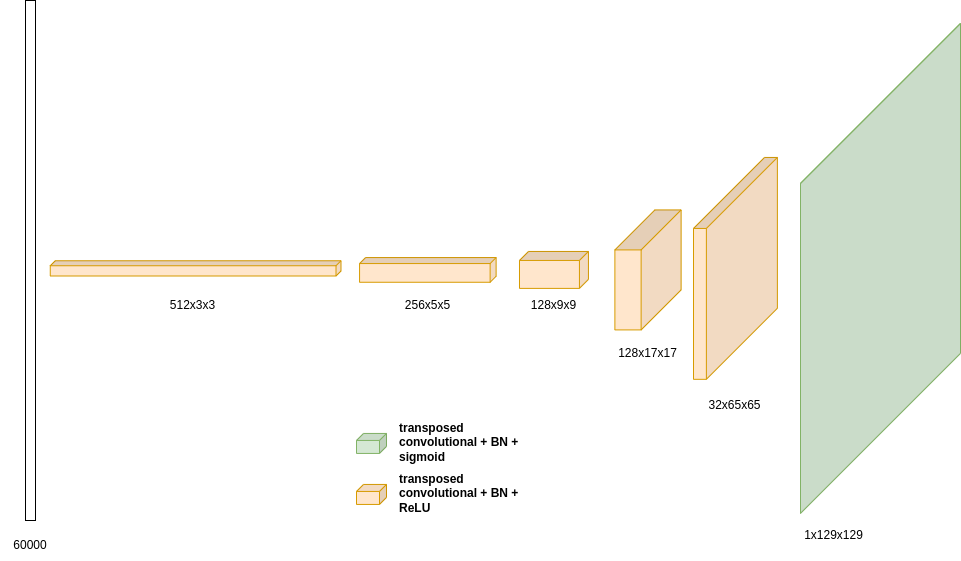
\includegraphics[width=140mm]{img/cnnv1.drawio.png}
\caption{First version of the CNN architecture simply takes the input and uses only transpose convolutional layers without any linear layers to produce the output.}
\label{img:methods:models:CNNv1}
\end{figure}


% **************************************************
\subsection{CNNv2}
\label{methods:models:CNNv2}
The second model is a CNN-based model with a total of 2 sequential parts.

The first part is a fully connected layer consisting of a linear transformation followed by batch normalization, ReLU activation, and dropout. The second part is a sequence of 6 transpose convolutional layers, also known as deconvolutional layers, followed by batch normalization and ReLU activation, and the final layer is a sigmoid activation function. 

The second part of the model takes an input tensor of size [B, 64, 8, 8] and outputs a tensor of size [B, 1, 289, 289], where $B$ is the batch size. The model has a total of 34,695,873 trainable parameters. Since the output is not 110x110px, we again use the same approach by adding bilinear interpolation to create the required output size. The architecture is drawn on picture~\ref{img:methods:models:CNNv2}.

\begin{figure}[H]\centering
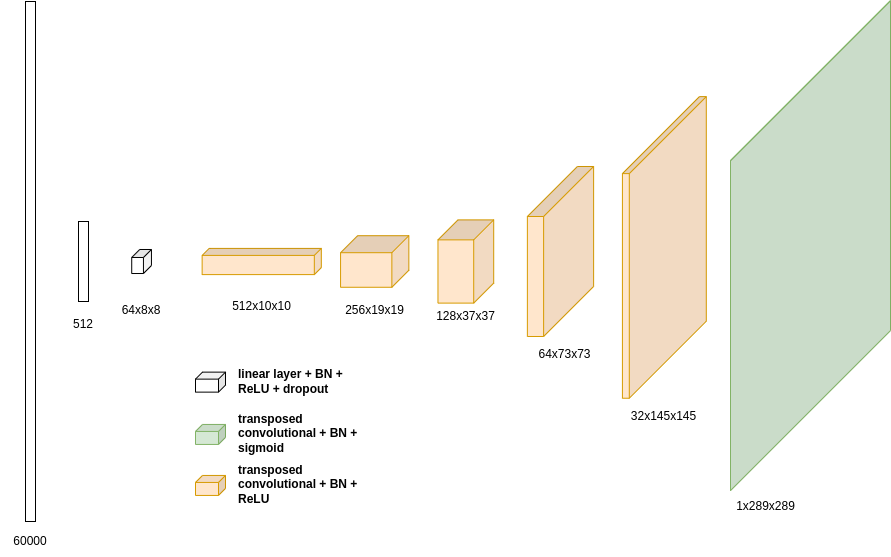
\includegraphics[width=140mm]{img/cnnv2.drawio.png}
\caption{Second version of the CNN architecture. This architecture contains a linear-encoding part and a decoding part producing the final output.}
\label{img:methods:models:CNNv2}
\end{figure}


% **************************************************
\subsection{CNNv3}
\label{methods:models:CNNv3}
The third generative model designed to produce images consists of two main components: a fully connected neural network and a convolutional neural network.

The fully connected network takes a cortical activity vector as input and outputs a 12100-dimensional feature vector. The feature vector is then reshaped into a 110x110px intermediate image tensor and passed through a series of transposed convolutional layers. These layers preserve the spatial dimensions and gradually decrease the channel resolution of the tensor until it has the same dimensions as the desired output image. 

The final layer of the convolutional neural network is a sigmoid activation function that squashes the pixel values of the output image to the range [0, 1]. This property is consistent across all of our models. This model has 38,527,629 trainable parameters and generates images with a size of 110x110 pixels exactly. This architecture is shown in picture~\ref{img:methods:models:CNNv3}.

\begin{figure}[H]\centering
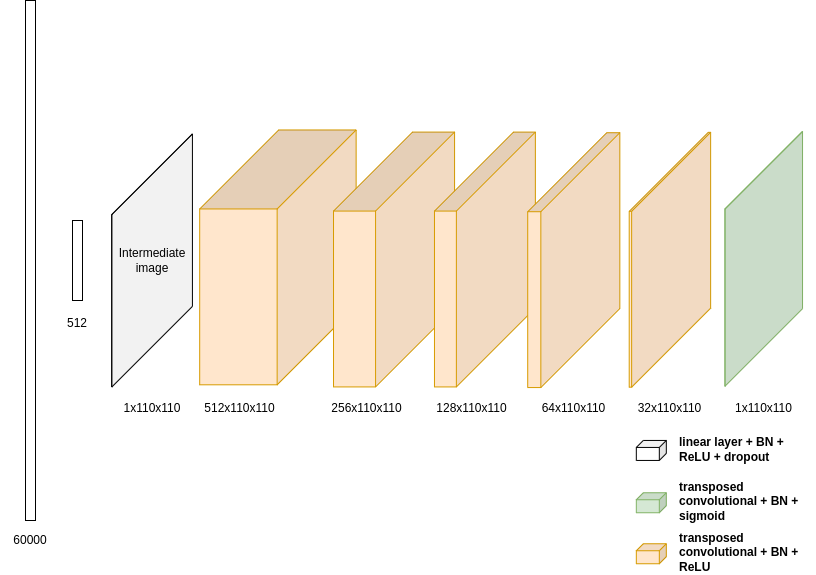
\includegraphics[width=140mm]{img/cnnv3.drawio.png}
\caption{Third version of the CNN architecture. Since the creation of the intermediate image, the dimensions stay the same except for the number of channels.}
\label{img:methods:models:CNNv3}
\end{figure}


% **************************************************
\subsection{CNNv4}
\label{methods:models:CNNv4}
This is a fourth CNN model for image generation, it is an implementation from paper~\citep{zhang2020reconstruction}\footnote{A detailed implementation code in Keras is available at \url{https://github.com/jiankliu/Spike-Image-Decoder/blob/main/SID.py}}. It consists of three sequential blocks. The first block is a fully connected neural network with two linear layers, batch normalization, ReLU activation, and dropout. This produces an intermediate image of size 110x110 pixels with a sigmoid activation function. The second block is a convolutional neural network with four convolutional layers, batch normalization, ReLU activation, and dropout. The third block is an upsampling neural network with four upsampling layers, four convolutional layers, batch normalization, ReLU activation, and dropout.

The input to this model is again a vector of cortical activity, and the output is an image of size 110x110 with each pixel between values 0 and 1. The model is using the sigmoid function as the final activation function to produce the output image. This architecture is drawn on picture~\ref{img:methods:models:CNNv4}.

The model has a total of 37,107,157 parameters out of which 30,720,512 parameters are contained in the first block containing linear layers.

\begin{figure}[H]\centering
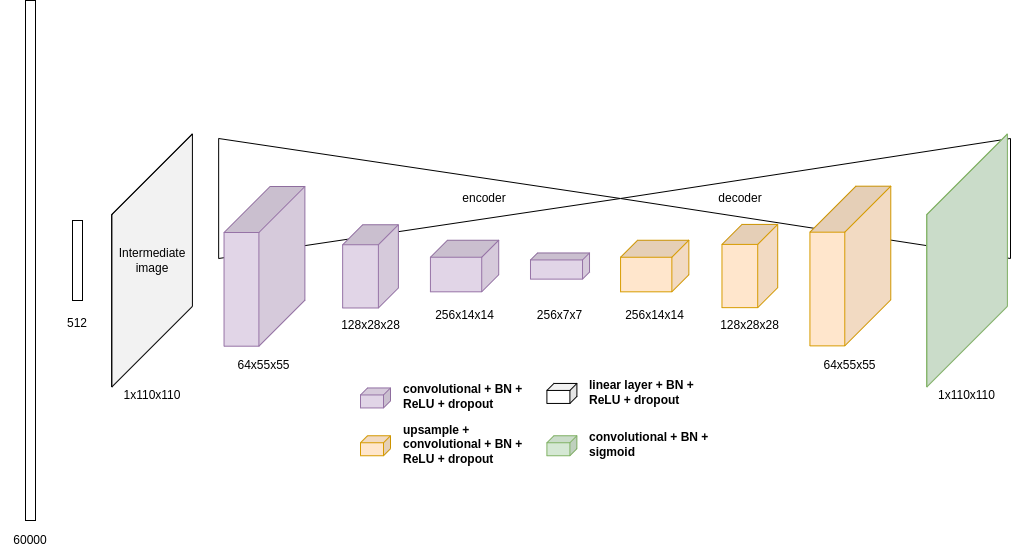
\includegraphics[width=140mm]{img/cnnv4.drawio.png}
\caption{Fourth version of the CNN architecture. The first part producing the intermediate image is here easily distinguishable from the encoder-decoder part of the architecture.}
\label{img:methods:models:CNNv4}
\end{figure}




% ==================================================
\section{Losses}
\label{methods:losses}
To train the generator function~\ref{equation:predictor-loss-minimization}, we tried several loss functions $\SL$ that are commonly used for image restoration~\citep{zhao2016loss}. It is not clear which one is optimal: since the resulting image will be evaluated by a human observer, as we need to use perceptually motivated losses. Sometimes, multiple loss functions are combined to produce a more sophisticated one~\citep{zhao2016loss}. In our experiments, the loss functions are used both for training and evaluation as \textit{accuracy} metrics.


% **************************************************
\subsection{L1}
\label{methods:losses:L1}

$L_1$ loss, also known as the mean absolute error (MAE), is a measure of the difference between two continuous variables. This loss function can be used in regression analysis to evaluate the accuracy of a predictive model.

The $L_1$ loss of the predicted value $\hat{y}$ and the true value $y$ is defined as:

\begin{equation}
L_1(\hat{y},y) = |\hat{y} - y|\:.
\end{equation}

The $L_1$ loss is a pixel-wise loss that computes the absolute difference between predicted and true values, which is then averaged across pixels.  It has the property of being robust to outliers, as the loss is not affected by large differences between the predicted and true values. The interpretability of this loss function is especially evident when compared with other loss functions that we use.


% **************************************************
\subsection{MSE}
\label{methods:losses:MSE}
Mean squared error (MSE) is a loss function used in regression analysis to evaluate the accuracy of a model. It measures the average squared difference between the predicted and true values.

The MSE between the predicted value $\hat{y}$ and the true value $y$ is defined as:

\begin{equation}
MSE(\hat{y},y) = (\hat{y} - y)^2\:.
\end{equation}

The squared difference between the predicted and true values penalizes large errors more than small errors. It is another possible choice for regression problems where the goal is to minimize the average squared difference between the predicted and true real values. This loss function is computed pixel-wise and then averaged across all the pixels.


% **************************************************
\subsection{SSIM}
\label{methods:losses:SSIM}
The structural similarity (SSIM) index is a popular loss function used in image processing to measure the similarity between two images. It compares the structural information of the images, including luminance, contrast, and structure. The first definition was presented in~\citep{wang2004image}.

The SSIM index between two images $x$ and $y$ is defined as:

\begin{equation}
SSIM(x,y) = \frac{(2\mu_x\mu_y + c_1)(2\sigma_{xy} + c_2)}{(\mu_x^2 + \mu_y^2 + c_1)(\sigma_x^2 + \sigma_y^2 + c_2)}\:,
\end{equation}

where $\mu_x$ and $\mu_y$ are the mean values of images $x$ and $y$, $\sigma_x$ and $\sigma_y$ are the standard deviations of images $x$ and $y$, and $\sigma_{xy}$ is the cross-covariance between $x$ and $y$. The constants $c_1$ and $c_2$ are small constants added to stabilize the division and are typically set to $c_1=(k_1L)^2$ and $c_2=(k_2L)^2$, where $L$ is the dynamic range of the pixel values and $k_1$ and $k_2$ are constants.

The SSIM index ranges between 0 and 1, where a value of 1 indicates perfect similarity between the two images.

The SSIM loss between two images $x$ and $y$ is defined as:

\begin{equation}
L_{SSIM}(x,y) = 1 - SSIM(x,y)\:.
\end{equation}

This measures the dissimilarity between the two images, with a value of 0 indicating perfect similarity.

The advantage over $L_1$~\ref{methods:losses:L1} or MSE~\ref{methods:losses:MSE} is that it takes into account the perceptual quality of the image, rather than just pixel-wise differences.
One of the disadvantages of this loss is the necessity to determine a window size/resolution scale, at which the loss is computed. This is solved by the MSSSIM loss~\ref{methods:losses:MSSSIM}.


% **************************************************
\subsection{MSSSIM}
\label{methods:losses:MSSSIM}
The multiscale structural similarity (MSSSIM) index is an extension of the SSIM index that takes into account the multi-scale nature of image perception. It was first defined in~\citep{wang2003multiscale}. It compares the structural information of images at different scales, providing a more accurate measurement of image similarity.

The MSSSIM index between two images $x$ and $y$ is defined as:

\begin{equation}
MSSSIM(x,y) = \frac{1}{n}\sum_{i=1}^{n} w_i \cdot SSIM(x_i, y_i)\:,
\end{equation}

where $n$ is the number of scales, $x_i$ and $y_i$ are the images at the $i$-th scale, and $w_i$ is a weight parameter that depends on the scale. The weights are typically chosen to be a Gaussian function of the scale, with the largest weight assigned to the lowest scale.

The MSSSIM loss between two images $x$ and $y$ is defined as:

\begin{equation}
L_{MSSSIM}(x,y) = 1 - MSSSIM(x,y)\:.
\end{equation}

This measures the dissimilarity between the two images, with a value of 0 indicating perfect similarity.

MSSSIM loss is commonly used as a loss function in deep learning algorithms for image processing tasks such as image denoising~\citep{bera2019lightweight}, super-resolution~\citep{min2023d}, and image restoration~\citep{zhao2016loss}. It is preferred over other loss functions such as mean squared error and SSIM as it provides a more accurate measurement of image similarity by taking into account the multi-scale nature of image perception.


% **************************************************
\subsection{MIX: a loss combining $L_1$ and MSSSIM}
\label{methods:losses:MIX}
Similarly as in~\citep{zhao2016loss}, we implemented also a loss combined from $L_1$~\ref{methods:losses:L1} and MSSSIM loss~\ref{methods:losses:MSSSIM}. In the paper, a Gaussian function is used to give more weight to the central part of the image for the $L_1$ loss. As we do not use this, in our case the final loss is defined as:


\begin{equation}
L_{MIX}(x,y) = \alpha \cdot L_{MSSSIM}(x,y) + (1 - \alpha) \cdot L_1(x,y)\:,
\end{equation}
where the value of $\alpha$ is set as described in the paper~\citep{zhao2016loss} to $0.84$.


% **************************************************
\subsection{Discriminator}
\label{methods:losses:adversarial}
We tried also a more sophisticated loss function common in training Generative Adversarial Networks (GANs)~\citep{goodfellow2014generative}, which was implemented using a CNN network. The discriminator network is responsible for determining whether the input image is real or fake. The use of discriminator loss has been shown to improve the quality of generated images~\citep{radford2015unsupervised, ledig2017photorealistic, wang2018highresolution}.

The model has multiple convolutional layers, with an increasing number of filters. The input image size is expected to be 110x110 pixels and the final output is a single value between 0 and 1, which represents the probability that the input image is real. The leaky ReLU activation function is used after each convolutional layer, except for the final layer where the sigmoid activation function is used to produce the probability score. The architecture is presented in picture~\ref{img:methods:losses:adversarial}.

The total number of trainable parameters in the model is 6,300,865.

If we define an objective function for the discriminator $\ell \colon \SX \rightarrow [0,1]$ as
\begin{equation}
  \label{equ:generator_quality_2}
  \begin{array}{rl}
  F_\ell(\#\omega_g,\#\omega_\ell) = \displaystyle\frac{1}{m}\sum_{j=1}^m \big(\log (1 - \ell(g( x^j; \#\omega_g); \#\omega_\ell )) + \log \ell( s^j; \#\omega_\ell) \big) \:,
  \end{array}
\end{equation}

where $s \in \SX$ is the desired stimuli image, $g$ is the generator function defined in~\ref{methods:models:problem-definition}, $\#\omega_g$ are its trained parameters and $\#\omega_\ell$ are the parameters of the discriminator function.

The output value of the discriminator $\ell(x; \#\omega_\ell)$ corresponds to the probability, that the image $x \in \SX$ is a real image, the value $1 - \ell(x; \#\omega_l)$ corresponds to the probability that the image $x \in \SX$ is a synthetic image generated by the generator function $g$. The convolutional network implementing the discriminator function contains a sigmoid function at the end to produce the probability.

We find the parameters $\#\omega_\ell$ and $\#\omega_g$ by solving a minimax problem:
\begin{equation}
   \label{equ:minimax}
    (\#\omega^*_g, \#\omega_\ell^*) \leftarrow \min_{\#\omega_g}\max_{\#\omega_\ell} 
    F_\ell(\#\omega_g, \#\omega_\ell) \:.
\end{equation}
To solve~\ref{equ:minimax}, we minimize~\ref{equ:generator_quality_2} with respect to $\#\omega_g$ when $\#\omega_\ell$ is fixed to find the best parameters for the generator function $g$ and alternate this step with maximization with respect to $\#\omega_\ell$ when we use fixed $\#\omega_g$ parameters to find the best parameters for the discriminator function $\ell$.

\begin{figure}[H]\centering
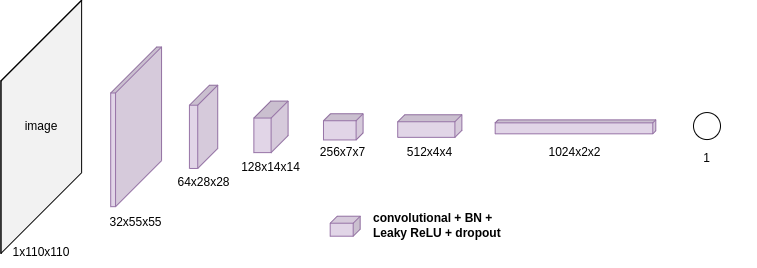
\includegraphics[width=140mm]{img/discriminator.drawio.png}
\caption{CNN architecture of the discriminator.}
\label{img:methods:losses:adversarial}
\end{figure}

To further improve the quality of the generated images, we use discriminator loss together with MSSSIM loss during training. The discriminator loss encourages the generated images to be indistinguishable from real images, while the MSSSIM forces the network to learn features that are based on the cortical activity. We selected a weights of $0.8$ for the discriminator loss and $0.2$ for the MSSSIM loss to balance the two objectives.




% ==================================================
\section{Implementation Details}
\label{methods:implementation-details}
To implement the methods, we used several Python libraries, which are available for both training the models and image augmentation or loss computation.

The linear regression models were trained using Python library scikit-learn\footnote{\url{https://scikit-learn.org}}, specifically using the class LinearRegression\footnote{\url{https://scikit-learn.org/stable/modules/generated/sklearn.linear_model.LinearRegression.html}}.

We implemented and trained the CNN models in the PyTorch\footnote{\url{https://pytorch.org}} framework. The settings for the training were selected as $0.0002$ for the learning rate, batch size of $64$, and the optimization was done using Adam optimizer~\citep{kingma2014adam}\footnote{PyTorch implementation is documented at \url{https://pytorch.org/docs/stable/generated/torch.optim.Adam.html}.} The number of epochs was $15$ (the best model was usually found after training the third epoch) and we used a cosine decay scheduler~\citep{loshchilov2016sgdr}, which starts at the given learning rate and follows the cosine function until it reaches zero learning rate.

For the computation of the loss functions, we used L1Loss and MSELoss implemented by PyTorch\footnote{\url{https://pytorch.org/docs/stable/generated/torch.nn.L1Loss.html} and \url{https://pytorch.org/docs/stable/generated/torch.nn.MSELoss.html}} and SSIMLoss and MS\_SSIMLoss implementations by popular Kornia\footnote{Kornia library is available at \url{https://kornia.github.io}.} library\footnote{\url{https://kornia.readthedocs.io/en/latest/_modules/kornia/losses/ssim.html} and \url{https://kornia.readthedocs.io/en/latest/_modules/kornia/losses/ms_ssim.html}}. All the other loss functions are either implemented in PyTorch or are combinations of these loss functions. The big advantage of these functions is that all of them can be run on GPU, which provides a speedup for their computation.
Note that the losses used for evaluation are computed only for the central 64x64 pixel area, as the reconstruction on the boundaries was not possible by any model we tried. The training loss was always computed for the whole image.

% ==================================================
% ==================================================
\chapter{Datasets}
\label{dataset}
For the thesis, a spiking model of a cat's primary visual cortex was used to generate the datasets~\citep{antolik2018comprehensive}. We used two main datasets, one smaller for initial experiments and one larger to fine-tune the CNN models. In general, we used zero mean, standard deviation one for normalization of cortical activity neurons and we divided the stimuli by $255$ to have all images in the range of $[0;1]$.


% ==================================================
\section{Ten-trials Dataset}
\label{dataset:ten-trials}
The use of a smaller dataset consisting of 10 image presentations per each image has its own advantages, despite having a smaller size. One of the intrinsic properties of neural responses is the presence of noise. By averaging the cortical activity across these 10 trials, the noise level can be reduced to some extent. Instead of averaging the results, we allowed the models to decide how to incorporate the noise into the learning process. We used this smaller dataset as a starting point to develop our generator models, but we found that it was insufficient to achieve satisfactory levels of accuracy. Therefore, we switched to using the larger dataset consisting of single-trial cortical activity responses (refer to dataset~\ref{dataset:one-trial}) to train the same models and do the rest of the experiments.


% **************************************************
\subsection{Preparation}
\label{dataset:ten-trials:preparation}
This dataset was obtained using a computational model of a cat's striate cortex, which was developed by Antolík and his colleagues~\citep{antolik2018comprehensive}. This in-silico model of cat's V1 is composed of a total of 60000 neurons, all of which are modeled as exponential integrate-and-fire point neurons~\citep{brette2005adaptive}. The neurons which are divided into layer 4 (L4), containing 30000 neurons, and layer 2/3 (L2/3), containing 30000 neurons. Moreover, the cortical neurons are divided into groups of excitatory and inhibitory neurons. The excitatory group of L4 contains 24000 neurons, the same holds for the excitatory group of L2/3. Both inhibitory groups of L4 and L2/3 contain 6000 neurons, therefore all four groups sum to 60000 neurons in total. Each neuron population presents particular inter-layer and intra-layer connectivity rules and specific physiological parameters in line with literature. In general, the model's design is heavily influenced by experimental findings and data measurements to ensure that the simulated spontaneous and visually evoked activity closely mimics the behavior of a real cat's V1.
Since this dataset was generated using a computational model, there are no limitations in terms of the number of trials that can be performed. The responses of 60000 neurons from layers L2/3 and L4 are included in the pairs of visual stimuli and neural population responses, which comprise resized and cropped grayscale images from ImageNet~\citep{russakovsky2015imagenet} with a resolution of 110x110 px. The responses are calculated by adding up the number of spikes that occur during a 560 ms time window aligned with the presentation of the stimulus. In this dataset, every image was presented to the model ten times.
Although each visual stimulus spans 11 degrees of the visual field, the cortical neurons are distributed only within a region of the cortex that corresponds to the 4 central degrees of the visual area covered by the stimuli. This decision was made to prevent boundary effects and allow for the complete receptive field of the cortical neurons to be accounted for. 


% **************************************************
\subsection{Description}
\label{dataset:ten-trials:description}

This dataset contains 5000 images in total. It contains each unique stimuli image ten times with different cortical activity encoding vector. For this reason, we split this dataset into training, validation, and testing part so that identical stimuli are always only inside one data part.
The samples consist of pairs of stimulus image, which has a shape of 110x110 pixels, and cortical activity neuron values, which are encoded as a vector with 60000 values.

The dataset was split with the rule 70:10:20 to produce the following number of samples in each part:


% --------------------------------------------------
\subsubsection{Training set}
\begin{itemize}
\item 3500 samples
\item Responses description: min $-0.813$, max $14.156$, mean $0$, std $1$
\item Stimuli description: min $0$, max $0.392$, mean $0.177$, std $0.104$
\end{itemize}


% --------------------------------------------------
\subsubsection{Validation set}
\begin{itemize}
\item 500 samples
\item Responses description: min $-0.813$, max $14.482$, mean $0.021$, std $1.027$
\item Stimuli description: min $0$, max $0.392$, mean $0.182$, std $0.107$
\end{itemize}


% --------------------------------------------------
\subsubsection{Testing set}
\begin{itemize}
\item 1000 samples
\item Responses description: min $-0.813$, max $12.731$, mean $0.002$, std $1.005$
\item Stimuli description: min $0$, max $0.392$, mean $0.182$, std $0.103$
\end{itemize}



% ==================================================
\section{One-trial Dataset}
\label{dataset:one-trial}
This is a much larger dataset, which was therefore more suitable to be used to develop and tune the CNN models.


% **************************************************
\subsection{Preparation}
\label{dataset:one-trial:preparation}
The dataset was prepared the same way as the one-trial dataset~\ref{dataset:ten-trials:preparation} except that each image was presented to the model only once, not ten times as in the previous dataset.


% **************************************************
\subsection{Description}
\label{dataset:one-trial:description}

The one-trial dataset contains unique stimuli images, therefore it could be simply split with the same 70:10:20 rule similar to the ten-trials dataset. In total, it contains 47250 samples.
The samples consist of pairs of stimulus image, which has a shape of 110x110 pixels, and cortical activity neuron values, which are encoded as a vector with 60000 values.

A detailed description of each part follows:

% --------------------------------------------------
\subsubsection{Training set}
\begin{itemize}
\item 33075 samples
\item Responses description: min $-1.045$, max $70.669$, mean $0$, std $1$
\item Stimuli description: min $0$, max $0.392$, mean $0.177$, std $0.106$
\end{itemize}

% --------------------------------------------------
\subsubsection{Validation set}
\begin{itemize}
\item 4725 samples
\item Responses description: min $-1.045$, max $31.697$, mean $0.001$, std $0.998$
\item Stimuli description: min $0$, max $0.392$, mean $0.178$, std $0.106$
\end{itemize}

% --------------------------------------------------
\subsubsection{Testing set}
\begin{itemize}
\item 9450 samples
\item Responses description: min $-1.045$, max $59.737$, mean $0.001$, std $1$
\item Stimuli description: min $0$, max $0.392$, mean $0.177$, std $0.107$
\end{itemize}

% ==================================================
% ==================================================
\chapter{Experiments}
\label{experiments}
This chapter outlines the experiments conducted to evaluate the performance of the LR and four presented CNN models on both the smaller and larger datasets. The experiments include testing different numbers of training samples to evaluate their impact on model performance and optimizing the number of input cortical neurons to optimize the models' number of parameters and identify the most important neurons. Additionally, we explore various loss functions to determine the most suitable for our problem. The main goal of these experiments is to identify the best model for accurately generating stimulus images from cortical activity.

In this chapter, we begin by describing the experiments conducted on the ten-trials dataset~\ref{experiments:ten-trials}. We evaluate the models using several loss functions to find the best model. Then we examine the dataset size by training several models~\ref{experiments:ten-trials:linear-regression} and explore the effect of intrinsic noise in the cortical neurons~\ref{experiments:ten-trials:intristic-noise-limitation}.

In the next section~\ref{experiments:one-trial}, we first evaluate the models using several loss functions and show the images generated by these models~\ref{experiments:one-trial:finding-best-model}. We also examine the intermediate images, which are used internally in the architecture of two of our models~\ref{experiments:one-trial:intermediate-image}. We then use the best model to find the best loss function for training the network~\ref{experiments:one-trial:finding-best-loss}. We also evaluate the dataset size and its influence on the $L_1$ loss value in section~\ref{experiments:one-trial:number-of-samples}. The number of neurons, which are available for training is high, therefore we try to use only subsets of these neurons first in section~\ref{experiments:one-trial:number-of-inputs}, where we use a random subset from the whole population. Later in section~\ref{experiments:one-trial:population-importance}, we compare the importance of different neuron population groups, as we are provided with the information from which group (L2/3, L4, and also inhibitory or excitatory) each neuron comes.
%In the latest section~\ref{experiments:one-trial:regularization}, we present several regularization techniques, that we try.


% ==================================================
\section{Ten-trials Dataset}
\label{experiments:ten-trials}
As a toy dataset, we used the small ten-trials dataset to see how the models will perform when the number of samples is very limited. Recall that the ten-trials dataset contains $3500$ samples for training, but each stimulus in this dataset is present ten-times. As a big advantage over the second and bigger one-trial dataset, this allows us to better capture the nature of the cortical activity, which is intristicaly noisy. The evaluation of the testing dataset is present in picture~\ref{img:experiments:ten-trials:comparison} using four different loss functions -- $L_1$, MSE, SSIM, and MSSSIM.

\begin{figure}[H]\centering
  \begin{subfigure}[t]{0.45\textwidth}
    \centering
    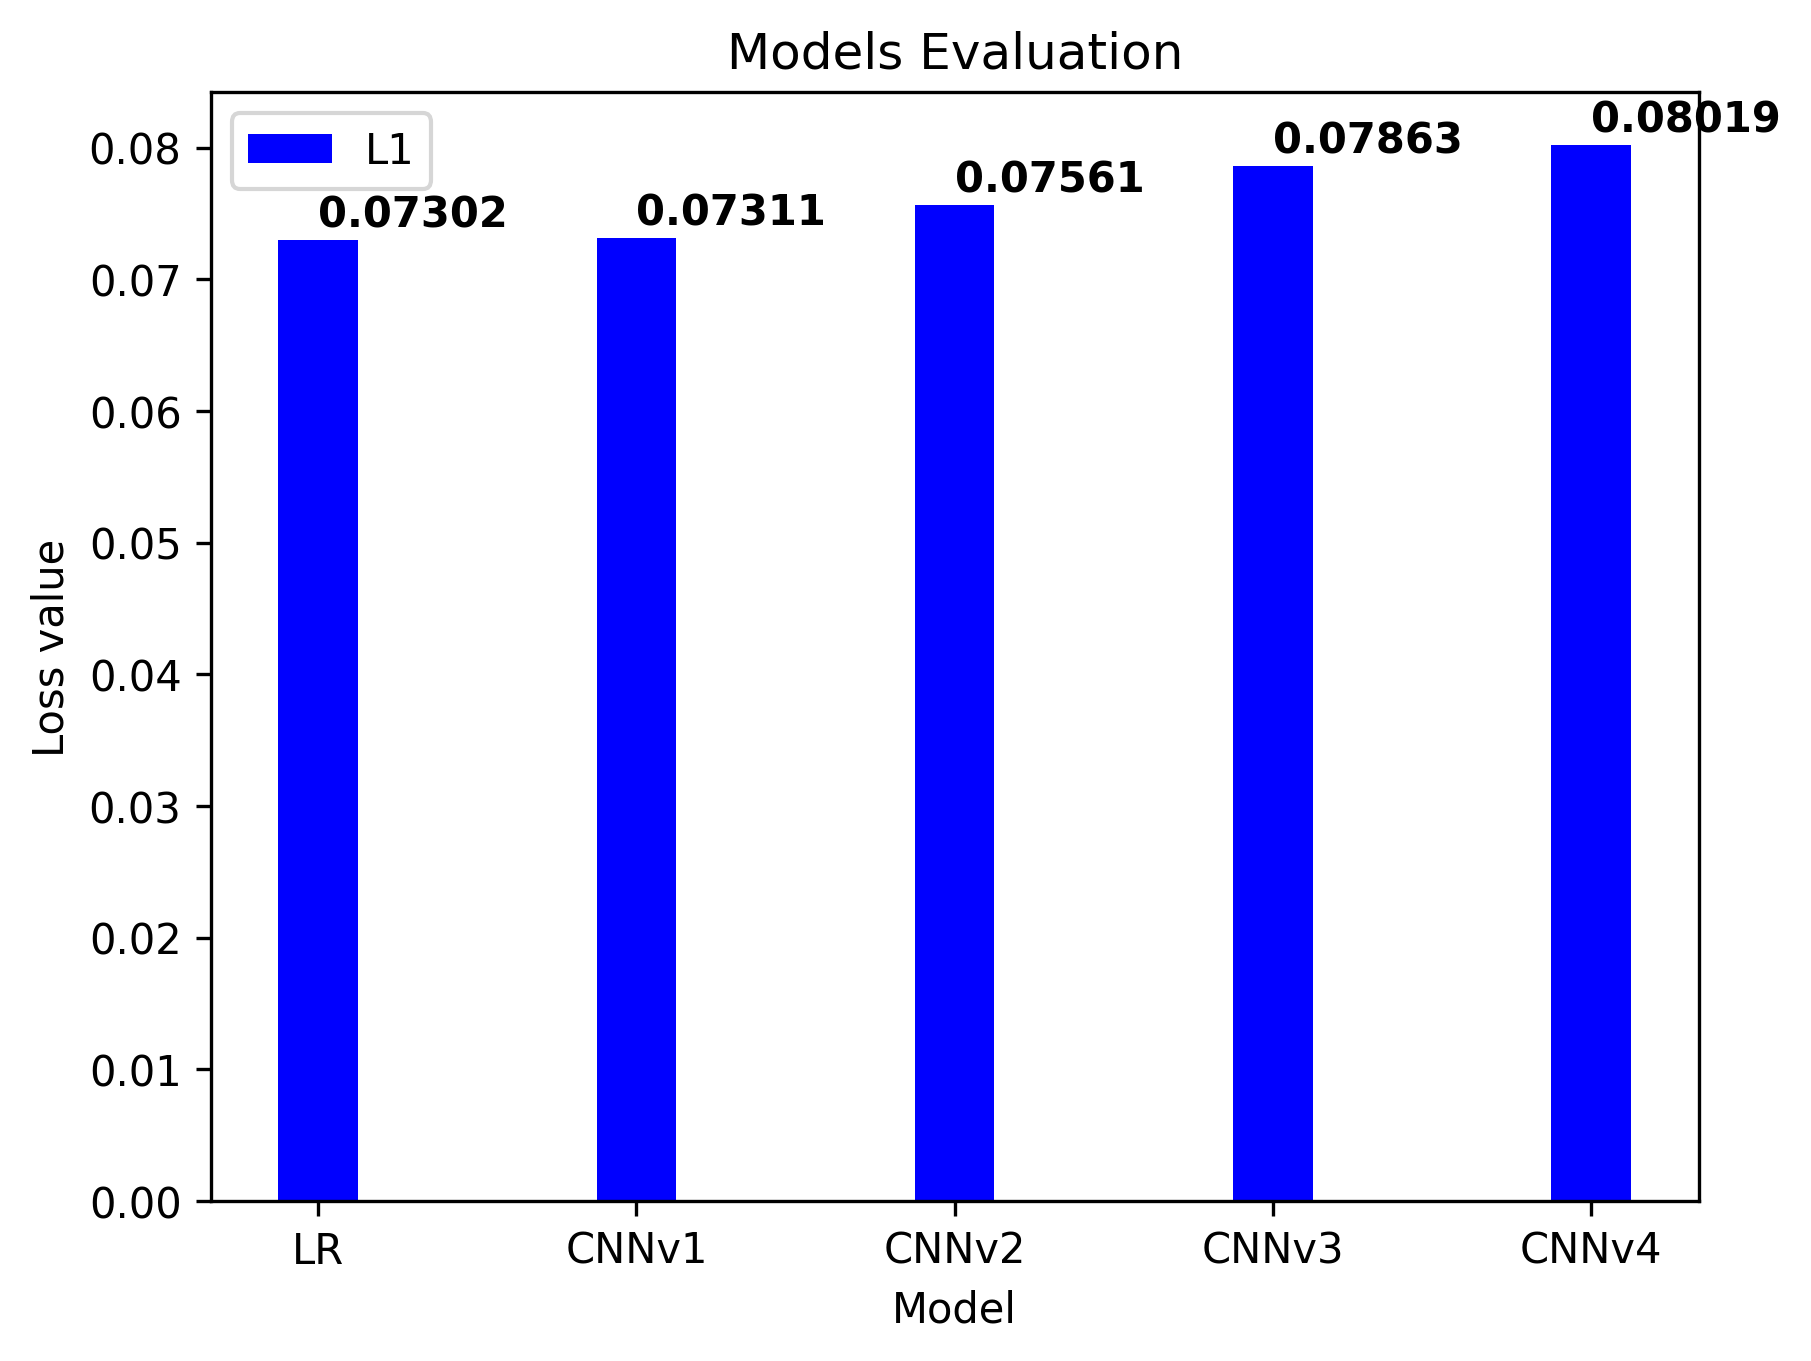
\includegraphics[width=\linewidth]{img/ten-trials/models_evaluation_ten_trials_l1.png}
    \caption{Models evaluation on $L_1$.}
  \end{subfigure}
  \begin{subfigure}[t]{0.45\textwidth}
    \centering
    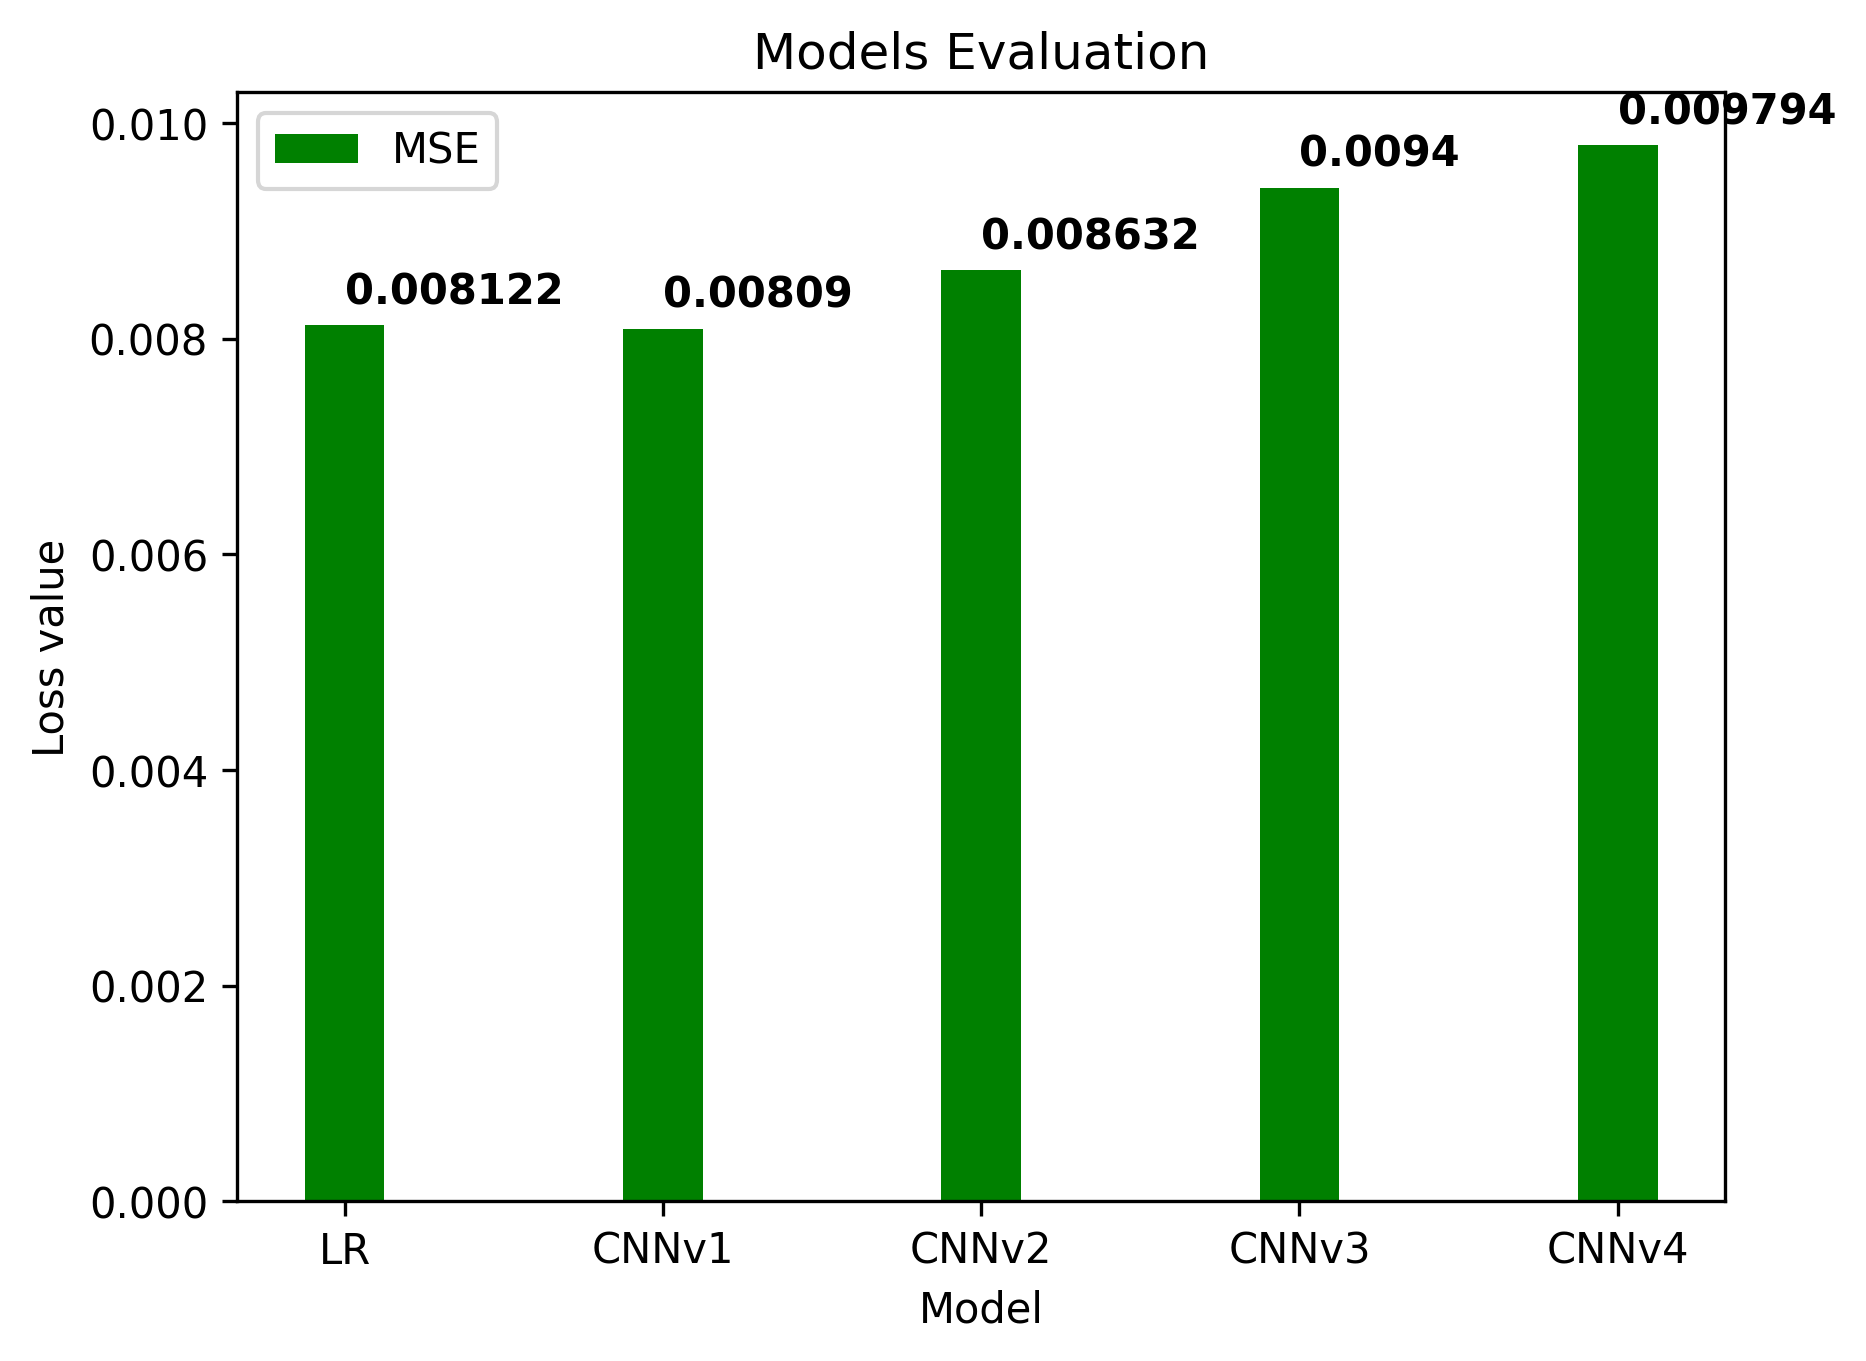
\includegraphics[width=\linewidth]{img/ten-trials/models_evaluation_ten_trials_mse.png}
    \caption{Models evaluation on MSE.}
  \end{subfigure}
  \\
  \begin{subfigure}[t]{0.45\textwidth}
    \centering
    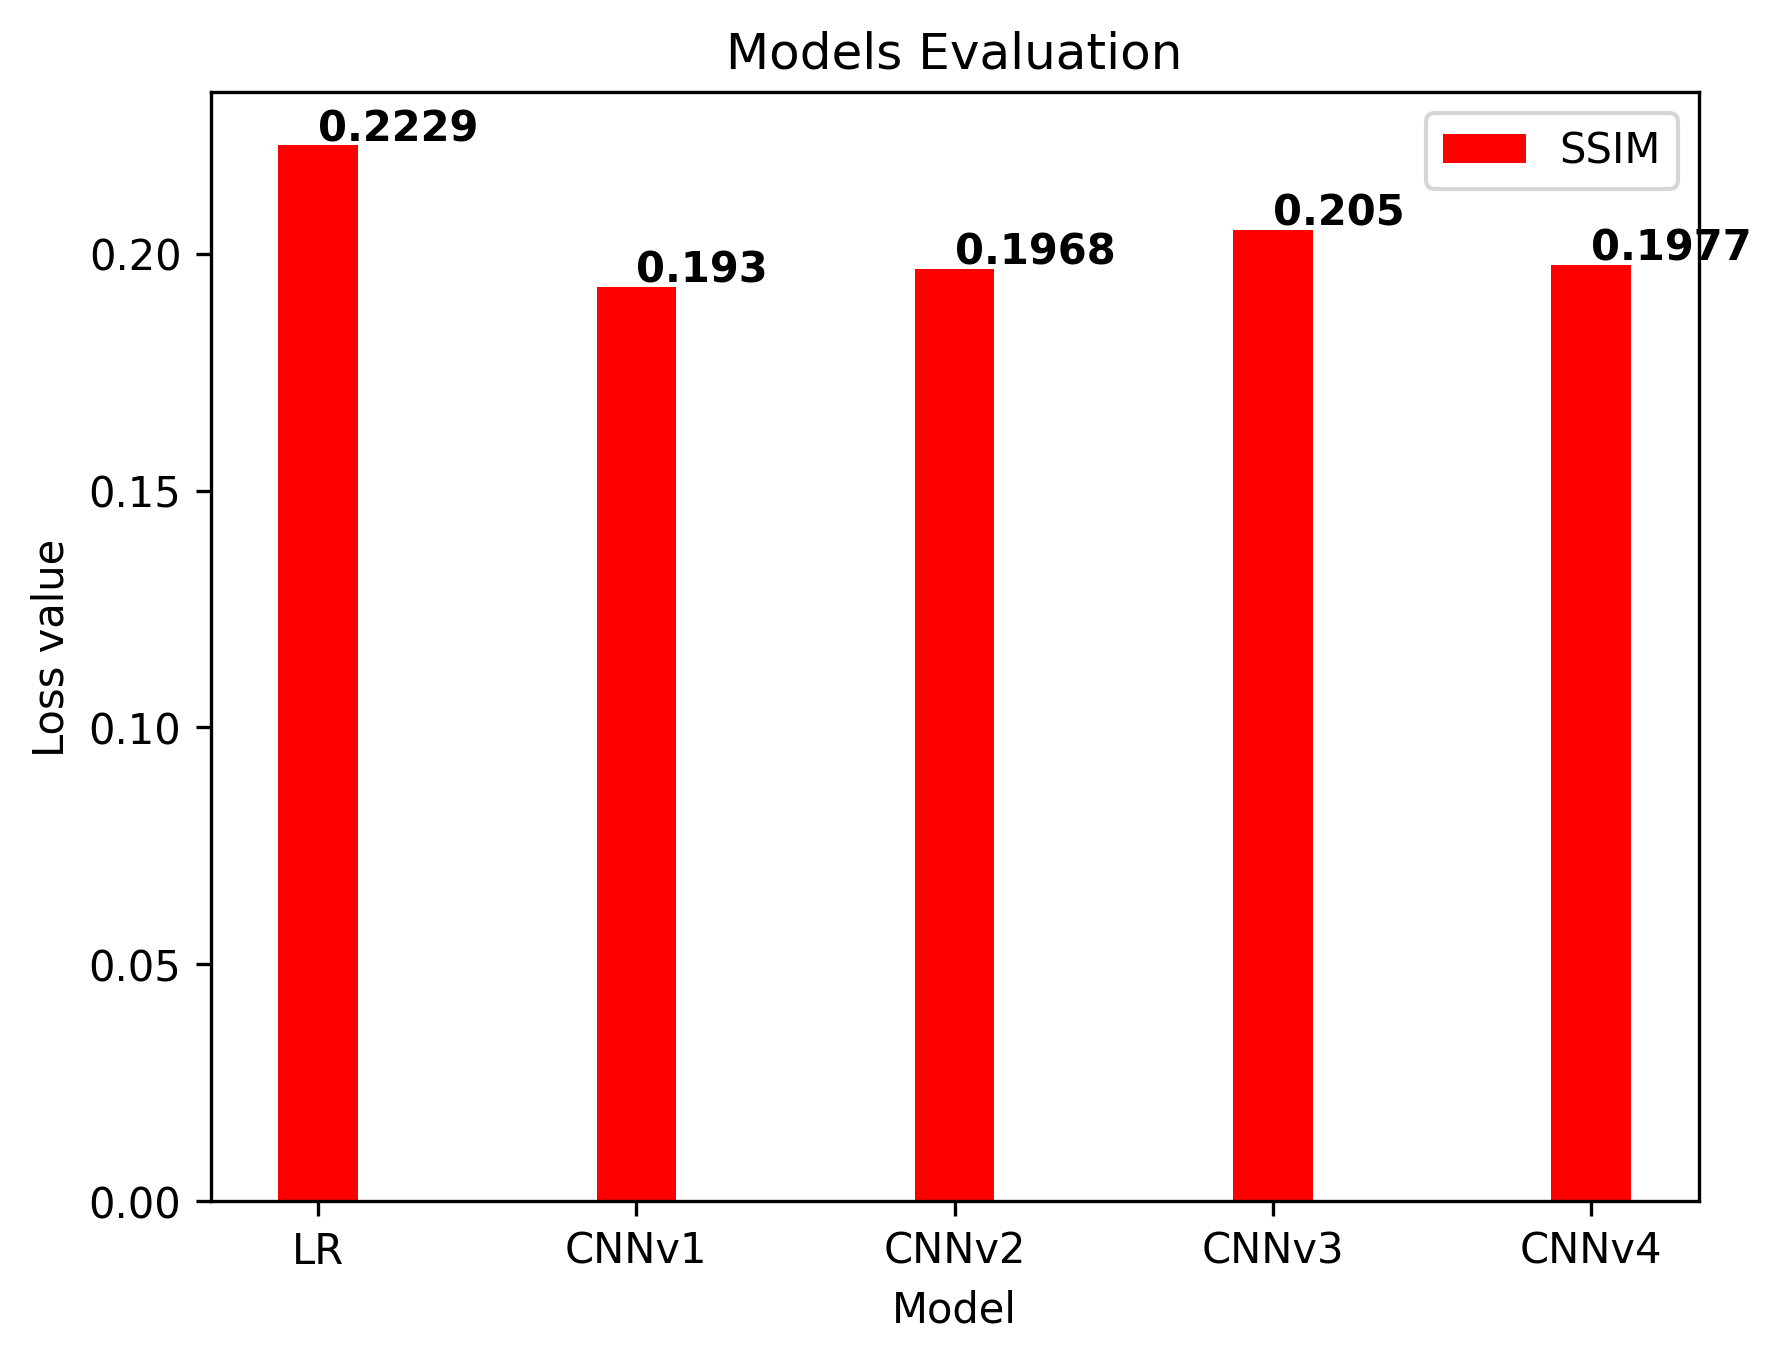
\includegraphics[width=\linewidth]{img/ten-trials/models_evaluation_ten_trials_ssim.png}
    \caption{Models evaluation on SSIM.}
  \end{subfigure}
  \begin{subfigure}[t]{0.45\textwidth}
    \centering
    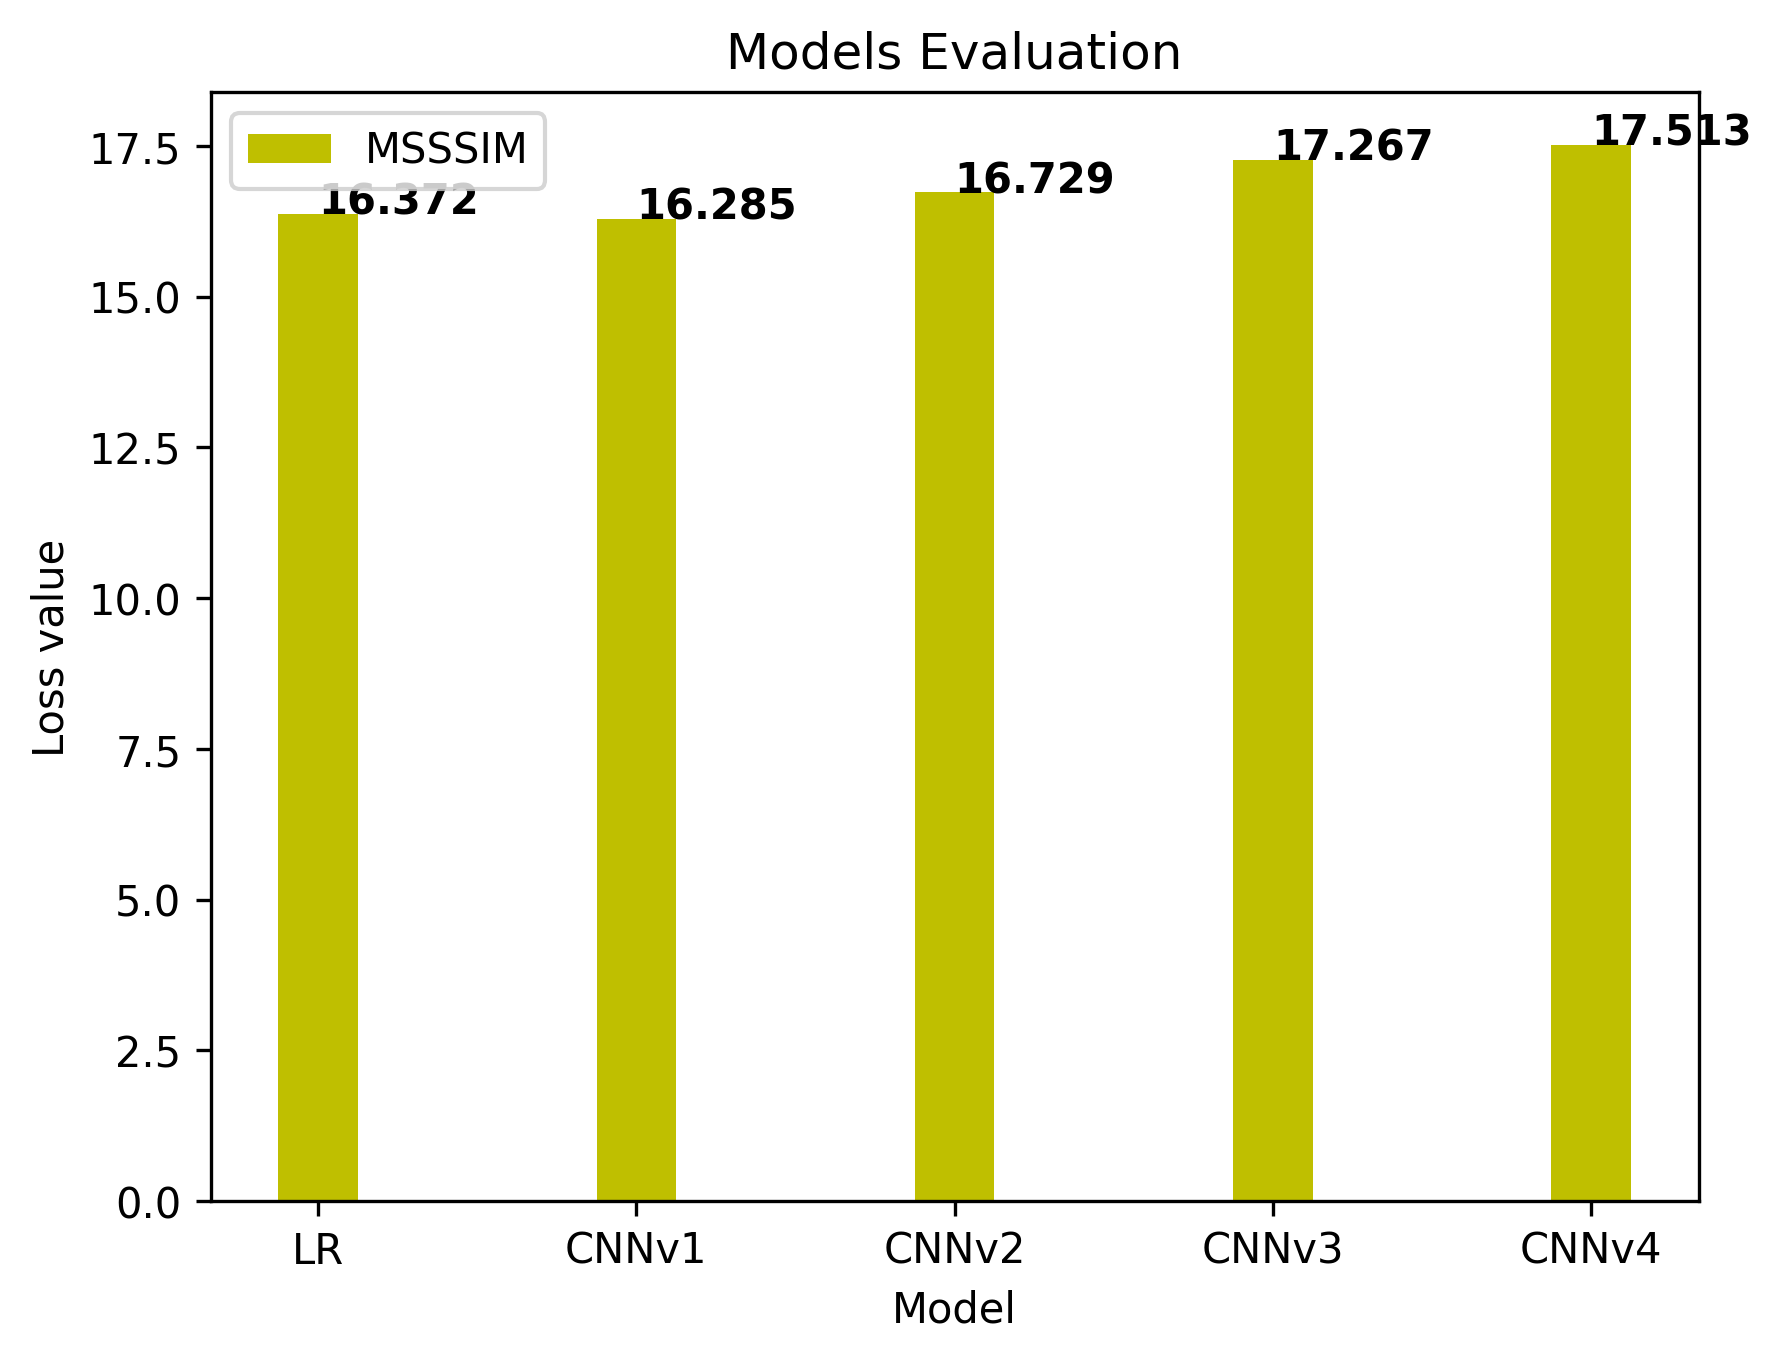
\includegraphics[width=\linewidth]{img/ten-trials/models_evaluation_ten_trials_msssim.png}
    \caption{Models evaluation on MSSSIM.}
  \end{subfigure}
  
%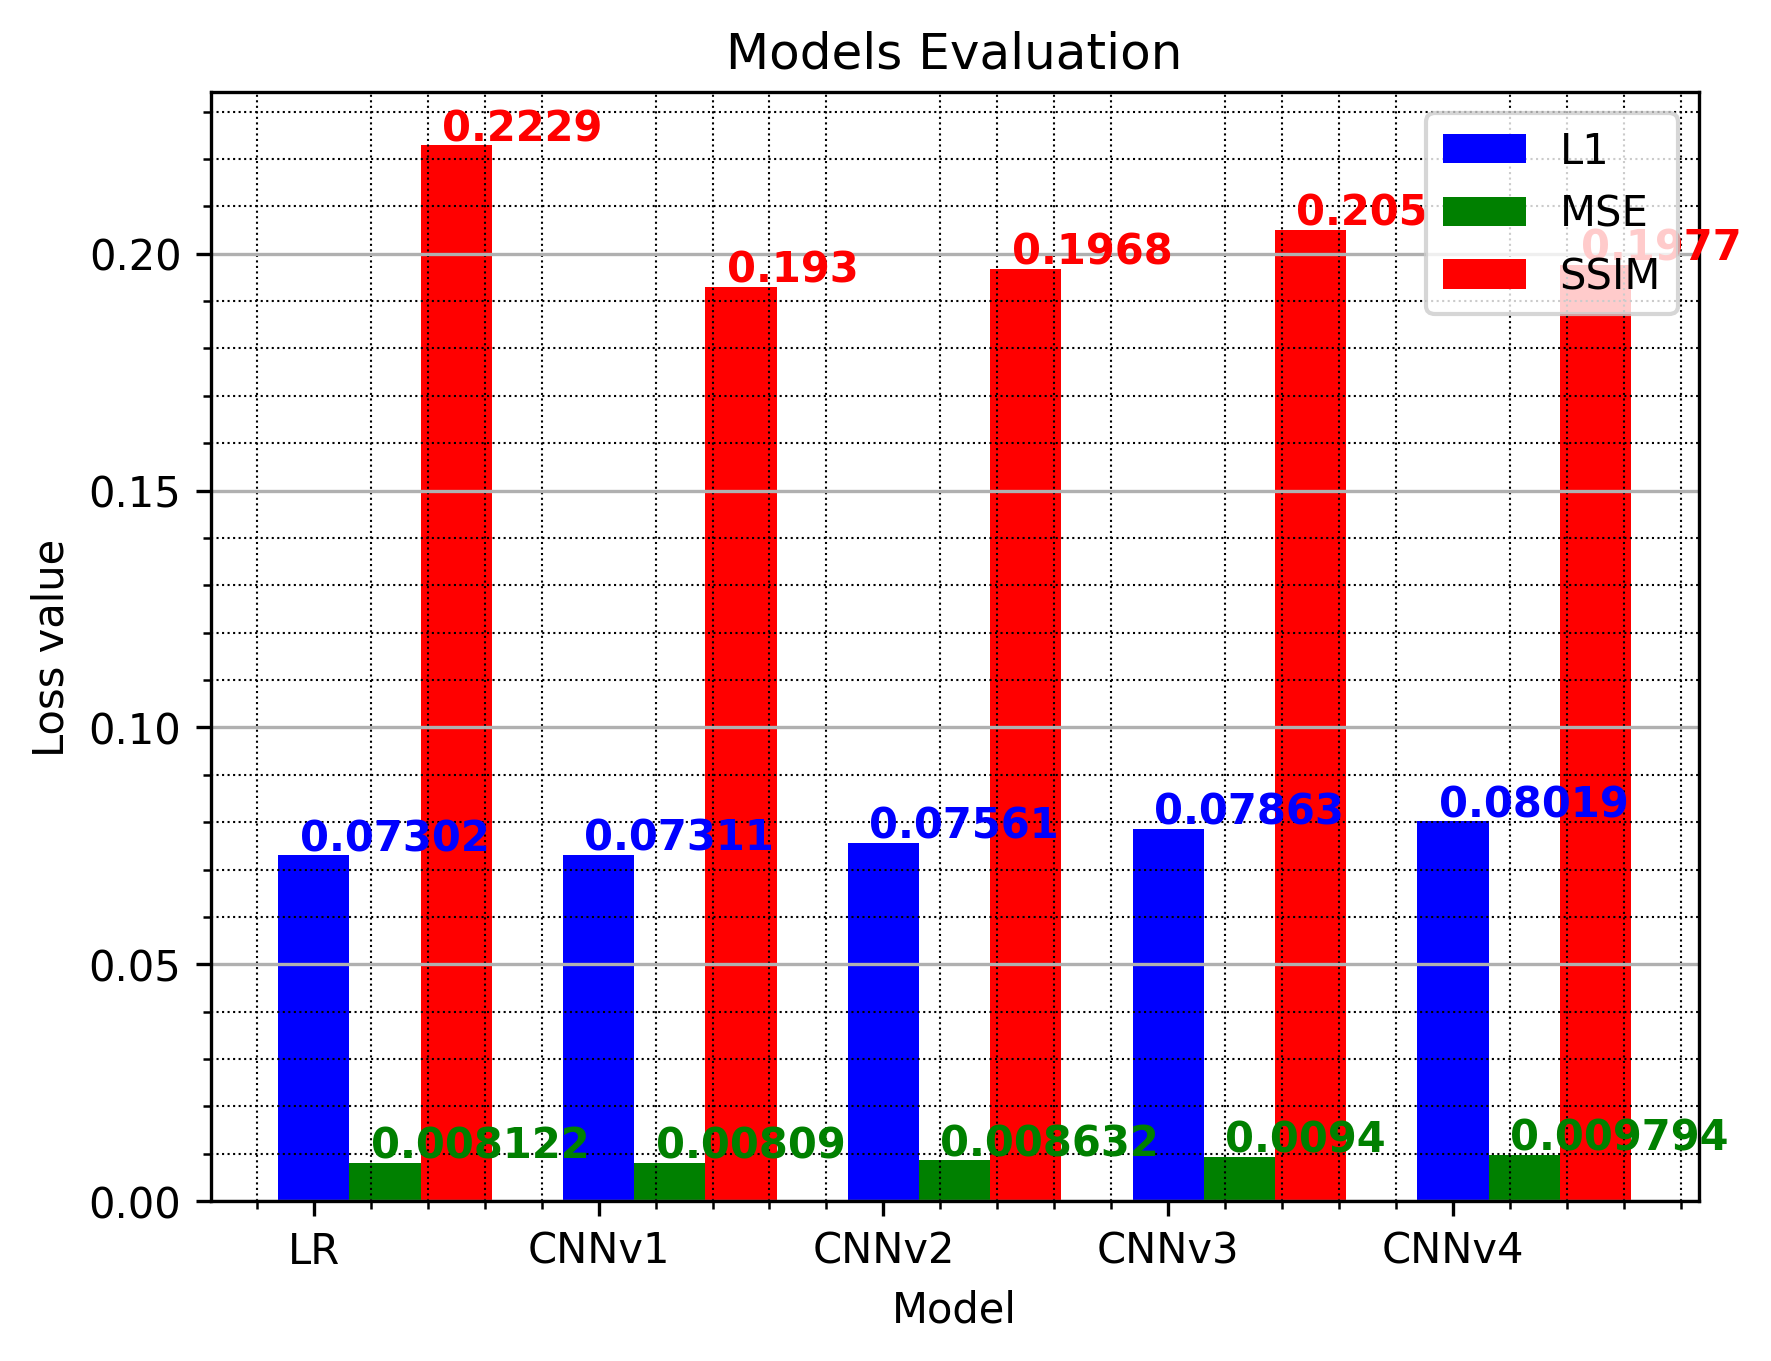
\includegraphics[width=140mm]{img/models_evaluation_ten_trials.png}
\caption{Comparison of multiple models on the same (one-trial) dataset using different loss metrics.}
\label{img:experiments:ten-trials:comparison}
\end{figure}

We can see that the linear regression (LR) and CNNv1 models compete for the lowest value in terms of $L_1$ (which is lowest for the CNNv1 model) and MSE (which is lowest for the LR model) but the values do not differ much and are comparable. The worst in terms of $L_1$ and MSE is the model CNNv4. You can compare the visual results on the testing dataset in the following image~\ref{img:experiments:ten-trials:comparison-outputs}.

\begin{figure}[H]\centering

  \begin{subfigure}[t]{0.15\textwidth}
    \centering
    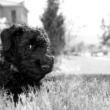
\includegraphics[width=\linewidth]{img/ten-trials/stimulus_1.png}
    %\caption{Stim. 1}
  \end{subfigure}
  \begin{subfigure}[t]{0.15\textwidth}
    \centering
    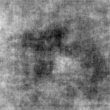
\includegraphics[width=\linewidth]{img/ten-trials/prediction_1_lr.png}
    % \caption{LR}
  \end{subfigure}
  \begin{subfigure}[t]{0.15\textwidth}
    \centering
    
\includegraphics[width=\linewidth]{img/ten-trials/prediction_1_cnnv1.png}
    % \caption{CNNv1}
  \end{subfigure}
  \begin{subfigure}[t]{0.15\textwidth}
    \centering
    
\includegraphics[width=\linewidth]{img/ten-trials/prediction_1_cnnv2.png}
    % \caption{CNNv2}
  \end{subfigure}
  \begin{subfigure}[t]{0.15\textwidth}
    \centering
    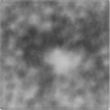
\includegraphics[width=\linewidth]{img/ten-trials/prediction_1_cnnv3.png}
    % \caption{CNNv3}
  \end{subfigure}
  \begin{subfigure}[t]{0.15\textwidth}
    \centering
    
\includegraphics[width=\linewidth]{img/ten-trials/prediction_1_cnnv4.png}
    % \caption{CNNv4}
  \end{subfigure}
  \\
    \vspace{0.1cm}
  
  \begin{subfigure}[t]{0.15\textwidth}
    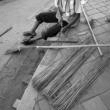
\includegraphics[width=\linewidth]{img/ten-trials/stimulus_2.png}
    \caption{Stimuli}
  \end{subfigure}
  \begin{subfigure}[t]{0.15\textwidth}
    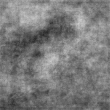
\includegraphics[width=\linewidth]{img/ten-trials/prediction_2_lr.png}
    \caption{LR}
  \end{subfigure}
  \begin{subfigure}[t]{0.15\textwidth}
    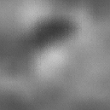
\includegraphics[width=\linewidth]{img/ten-trials/prediction_2_cnnv1.png}
    \caption{CNNv1}
  \end{subfigure}
  \begin{subfigure}[t]{0.15\textwidth}
    
\includegraphics[width=\linewidth]{img/ten-trials/prediction_2_cnnv2.png}
    \caption{CNNv2}
  \end{subfigure}
  \begin{subfigure}[t]{0.15\textwidth}
    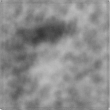
\includegraphics[width=\linewidth]{img/ten-trials/prediction_2_cnnv3.png}
    \caption{CNNv3}
  \end{subfigure}
  \begin{subfigure}[t]{0.15\textwidth}
    
\includegraphics[width=\linewidth]{img/ten-trials/prediction_2_cnnv4.png}
    \caption{CNNv4}
  \end{subfigure}
  
%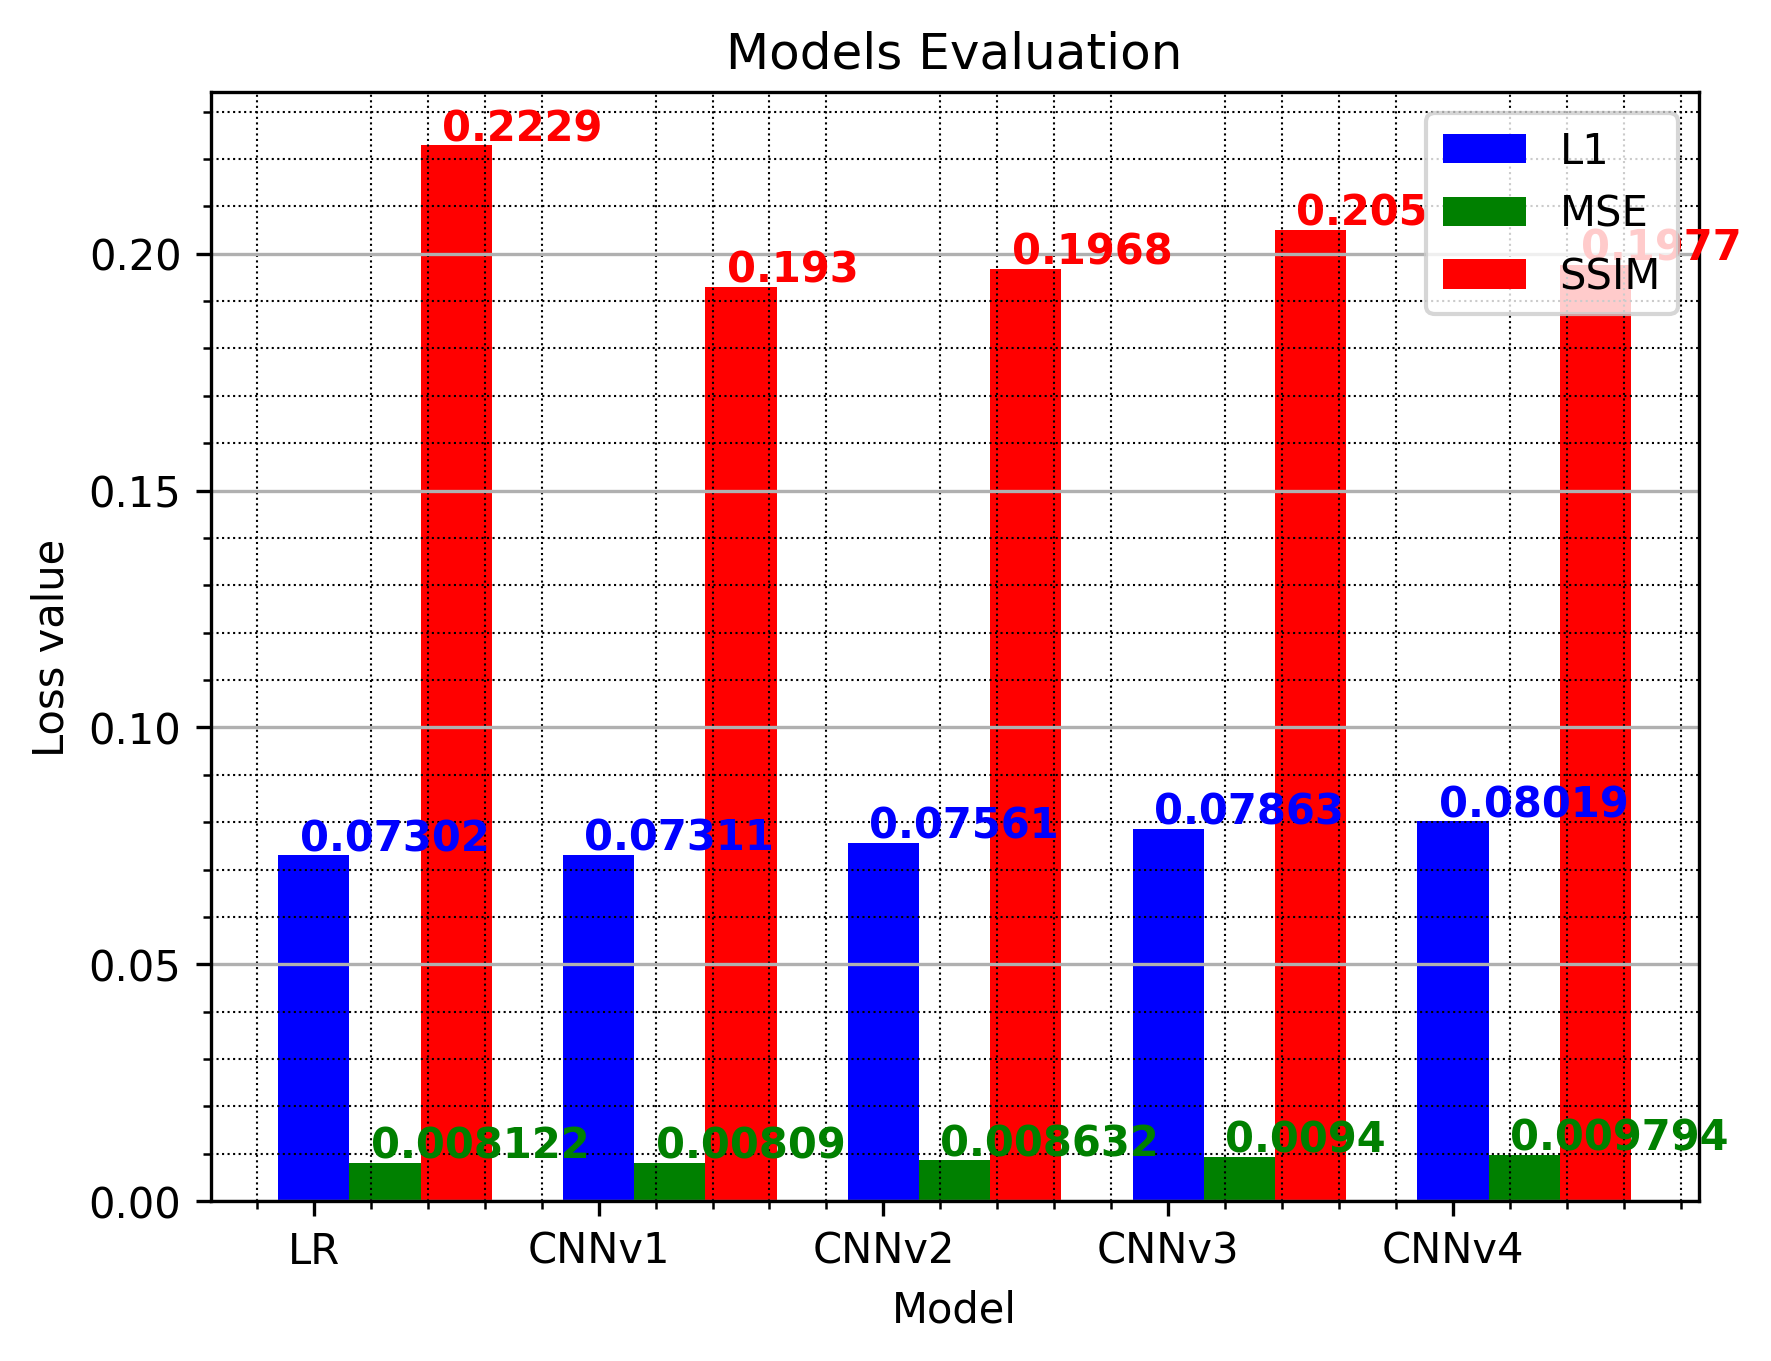
\includegraphics[width=140mm]{img/models_evaluation_ten_trials.png}
\caption{Comparison of multiple models on the same (ten-trials) dataset using different loss metrics.}
\label{img:experiments:ten-trials:comparison-outputs}
\end{figure}

On the image~\ref{img:experiments:ten-trials:comparison-outputs}, we see a comparison of the model outputs for two different cortical activity inputs on two testing samples. The first column contains the required stimulus image, and the rest of the columns correspond to each individual model. The second column to the linear regression model, the third one to CNNv1, and so on as described in the captions. We see that the LR and CNNv3 models try to reconstruct in a more detailed/localized way than the other models, although the reason of this behavior remains unclear.

All the models (except LR) were trained using MSSSIM loss (we present the reasons for using this loss in section~\ref{experiments:one-trial:finding-best-loss}). From the reconstructed images we can see, only a very limited number of low frequencies are being reconstructed. Interestingly, all the models, although independent, produce a similar reconstruction.


% **************************************************
\subsection{Linear Regression Dataset Size}
\label{experiments:ten-trials:linear-regression}
We tried to limit the number of data that were used to train the linear regression model~\ref{experiments:ten-trials:linear-regression}. We found that for this model, the loss function ($L_1$ in this case) value improved as the number of training data increased in the dataset until the maximum number of samples limit (3500 samples) was hit. We used linear regression for this task as the training is fully deterministic in comparison to CNN models, it is the fastest model to train on this dataset and the linear regression model performed best in terms of $L_1$, as described in~\ref{experiments:ten-trials}.

\begin{figure}[H]\centering
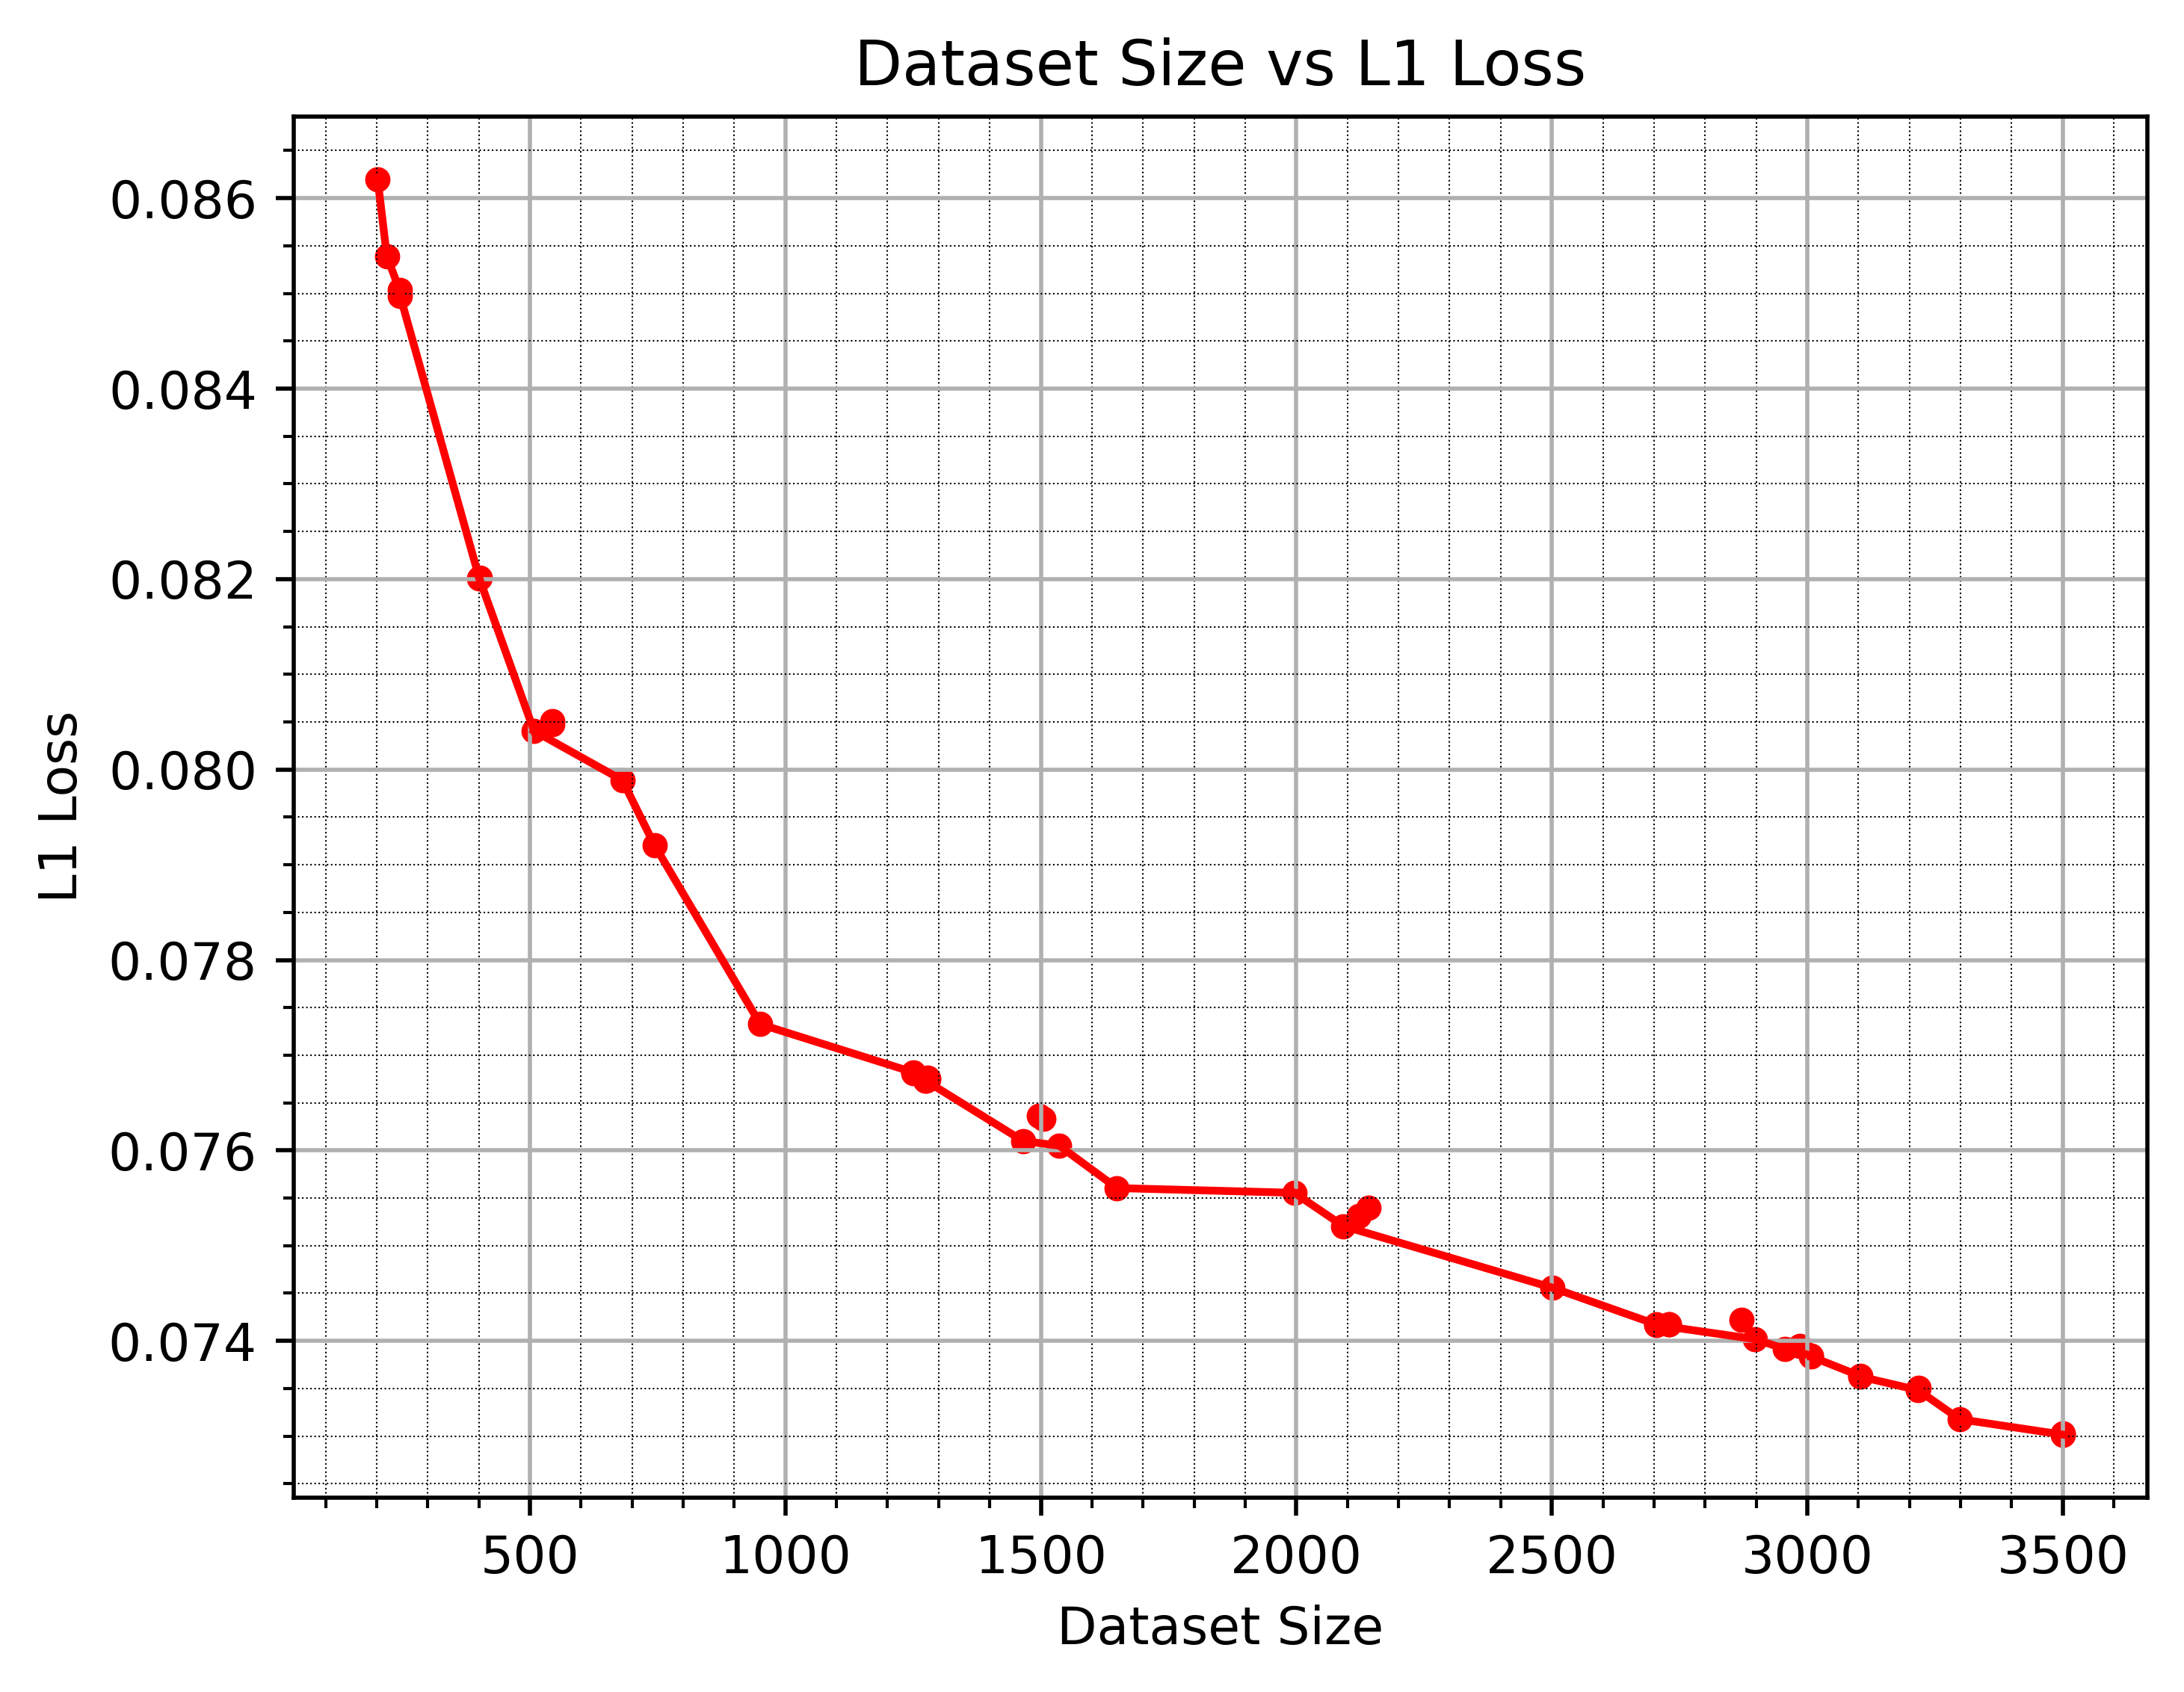
\includegraphics[width=140mm]{img/ten-trials/linear_regression_ten_trials.png}
\caption{Dependency of $L_1$ loss on the number of data in the training set for the linear regression model.}
\label{img:experiments:ten-trials:linear-regression}
\end{figure}

From this experiment, we conclude that the number of images is very important for the decoding of the stimuli. With a bigger dataset, it should be possible to perform better decoding.


% **************************************************
\subsection{Intristic Noise Limitation}
\label{experiments:ten-trials:intristic-noise-limitation}
To investigate if the intrinsic noise in neural responses represents a limitation for stimuli decoding, we used the best model for this dataset. Recall that we found that best model is the simple linear regression model (section~\ref{experiments:ten-trials}).

To find the answer to this question, use the following data:
\begin{description}
    \item[original] This dataset is unchanged, therefore contains each stimulus image ten-times with a different cortical response, meaning 3500 training samples (\ref{dataset:ten-trials}).
    \item[averaged] The same dataset, but the samples contain only unique stimuli images, each is crated by averaging the samples (responses) with the same stimulus image, therefore containing 350 samples for training. (The same is done for validation and testing samples.) The average is used here to remove the noise in the neural responses.
\end{description}

We then train two LR models:
\begin{enumerate}
    \item model, which is trained on all samples (\textbf{original} dataset)
    \item model, which is trained on averaged samples (\textbf{averaged} dataset)
\end{enumerate}

We already know, that the first model has $L_1$ loss of value $0.07304$ (\ref{experiments:ten-trials}). If we test the second model on the \textbf{averaged} dataset, we get $L_1$ value $0.07152$. From this, we conclude that the intristic noise in the neural responses represents a limitation for stimuli decoding, as we are able to get lower loss value by averaging the noisy samples across multiple trials. However, note that the improvement is not very significant.


% ==================================================
\section{One-trial Dataset}
\label{experiments:one-trial}
For the rest of the experiments, we will use the one-trial dataset~\ref{dataset:one-trial}, which is bigger than the ten-trials dataset and thus provides a better space for an improvement of the CNN models.


%% **************************************************
%\subsection{Linear Regression}
%\label{experiments:one-trial:linear-regression}
%\todo{description}


% **************************************************
\subsection{Finding Best Model}
\label{experiments:one-trial:finding-best-model}
To find the best-performing model, we trained all the model architectures described in~\ref{methods:models} on the training part of the one-trial dataset, we selected the best model state based on the validation part of the dataset and evaluated the results on the testing part of the dataset using the 4 main presented losses~\ref{methods:losses}.


\begin{figure}[H]\centering
  \begin{subfigure}[t]{0.45\textwidth}
    \centering
    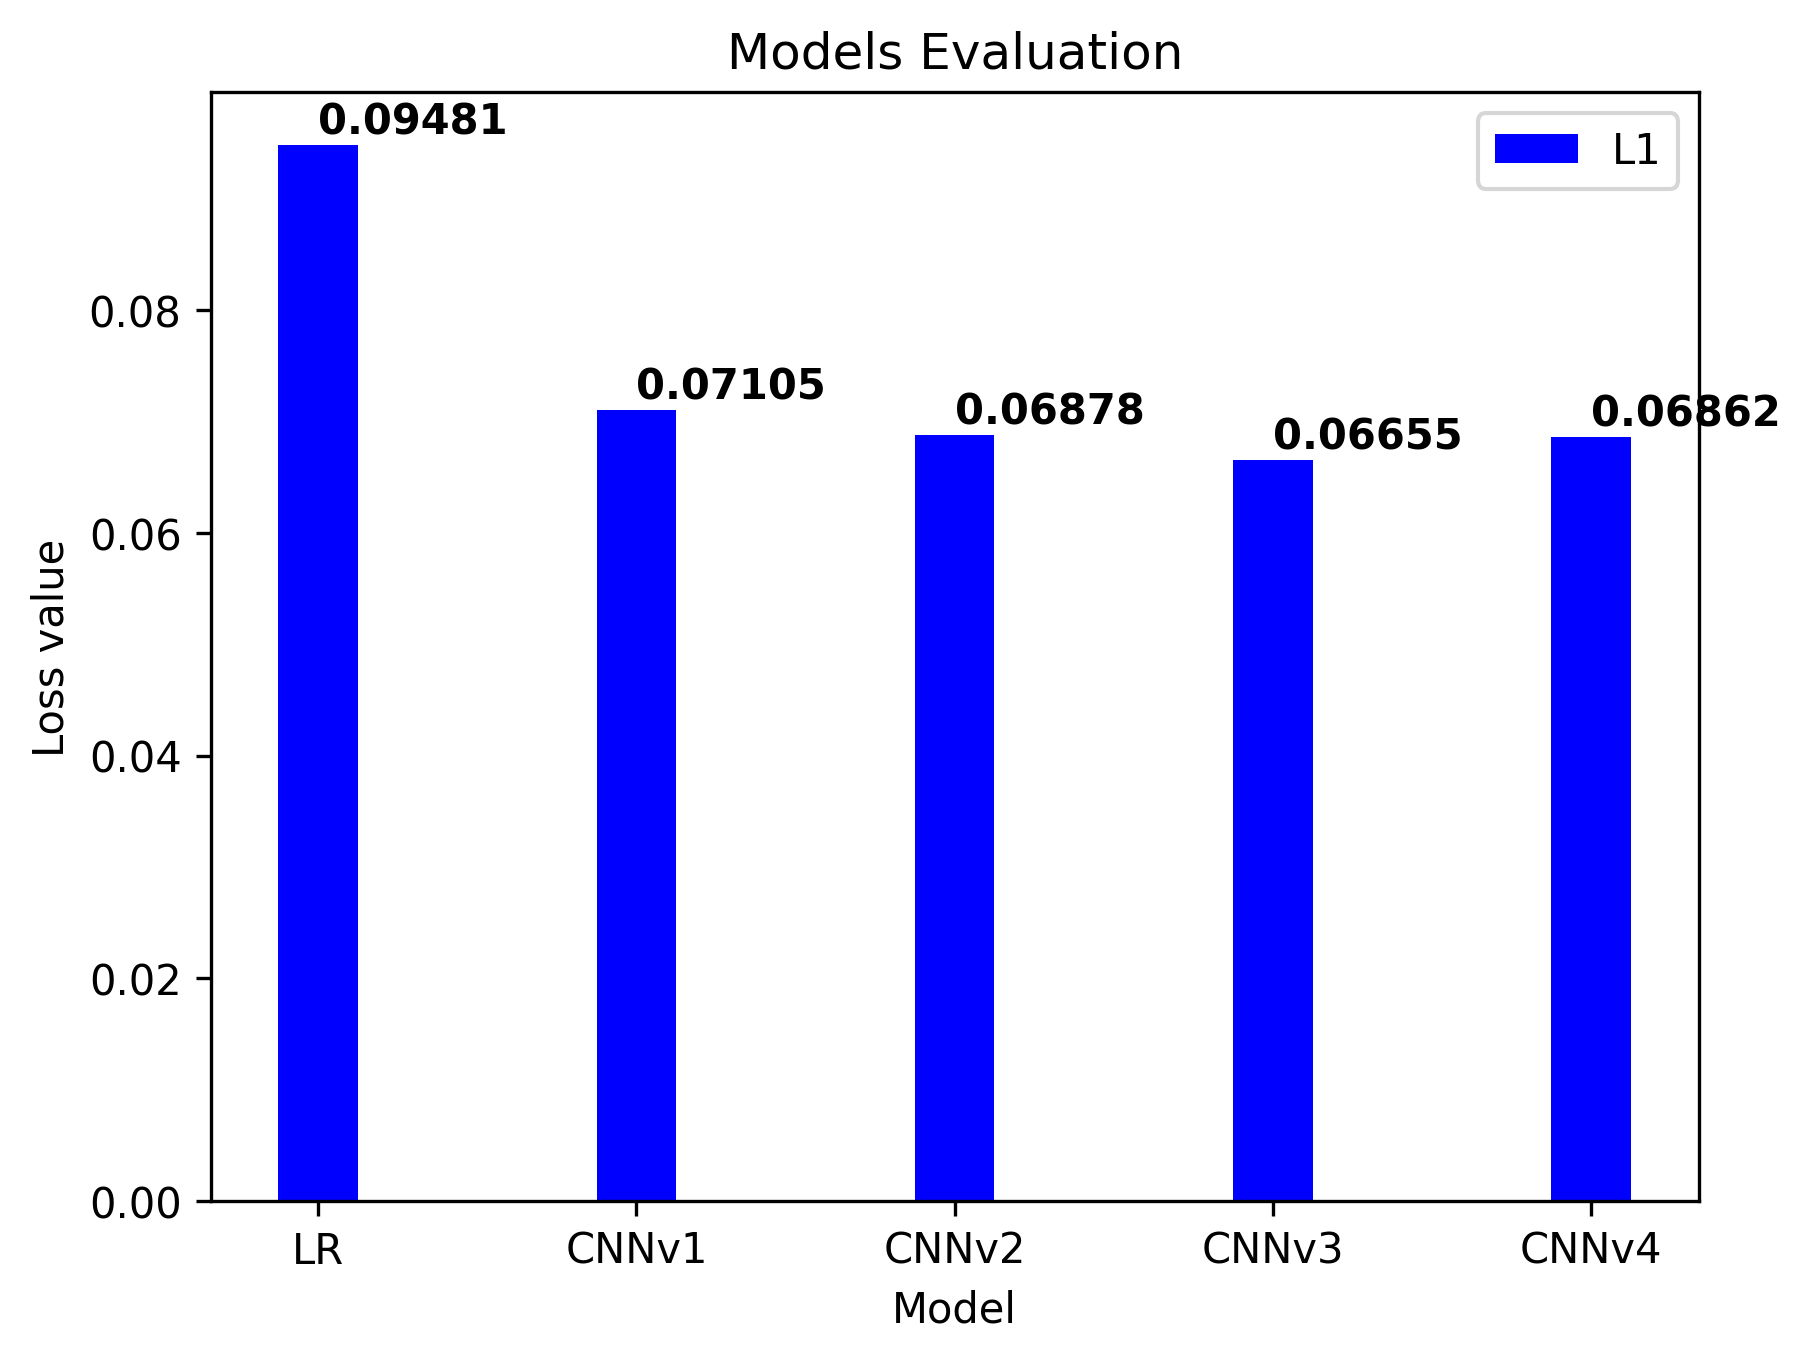
\includegraphics[width=\linewidth]{img/one-trial/models_evaluation_one_trial_l1.png}
    \caption{Models evaluation on $L_1$.}
  \end{subfigure}
  \begin{subfigure}[t]{0.45\textwidth}
    \centering
    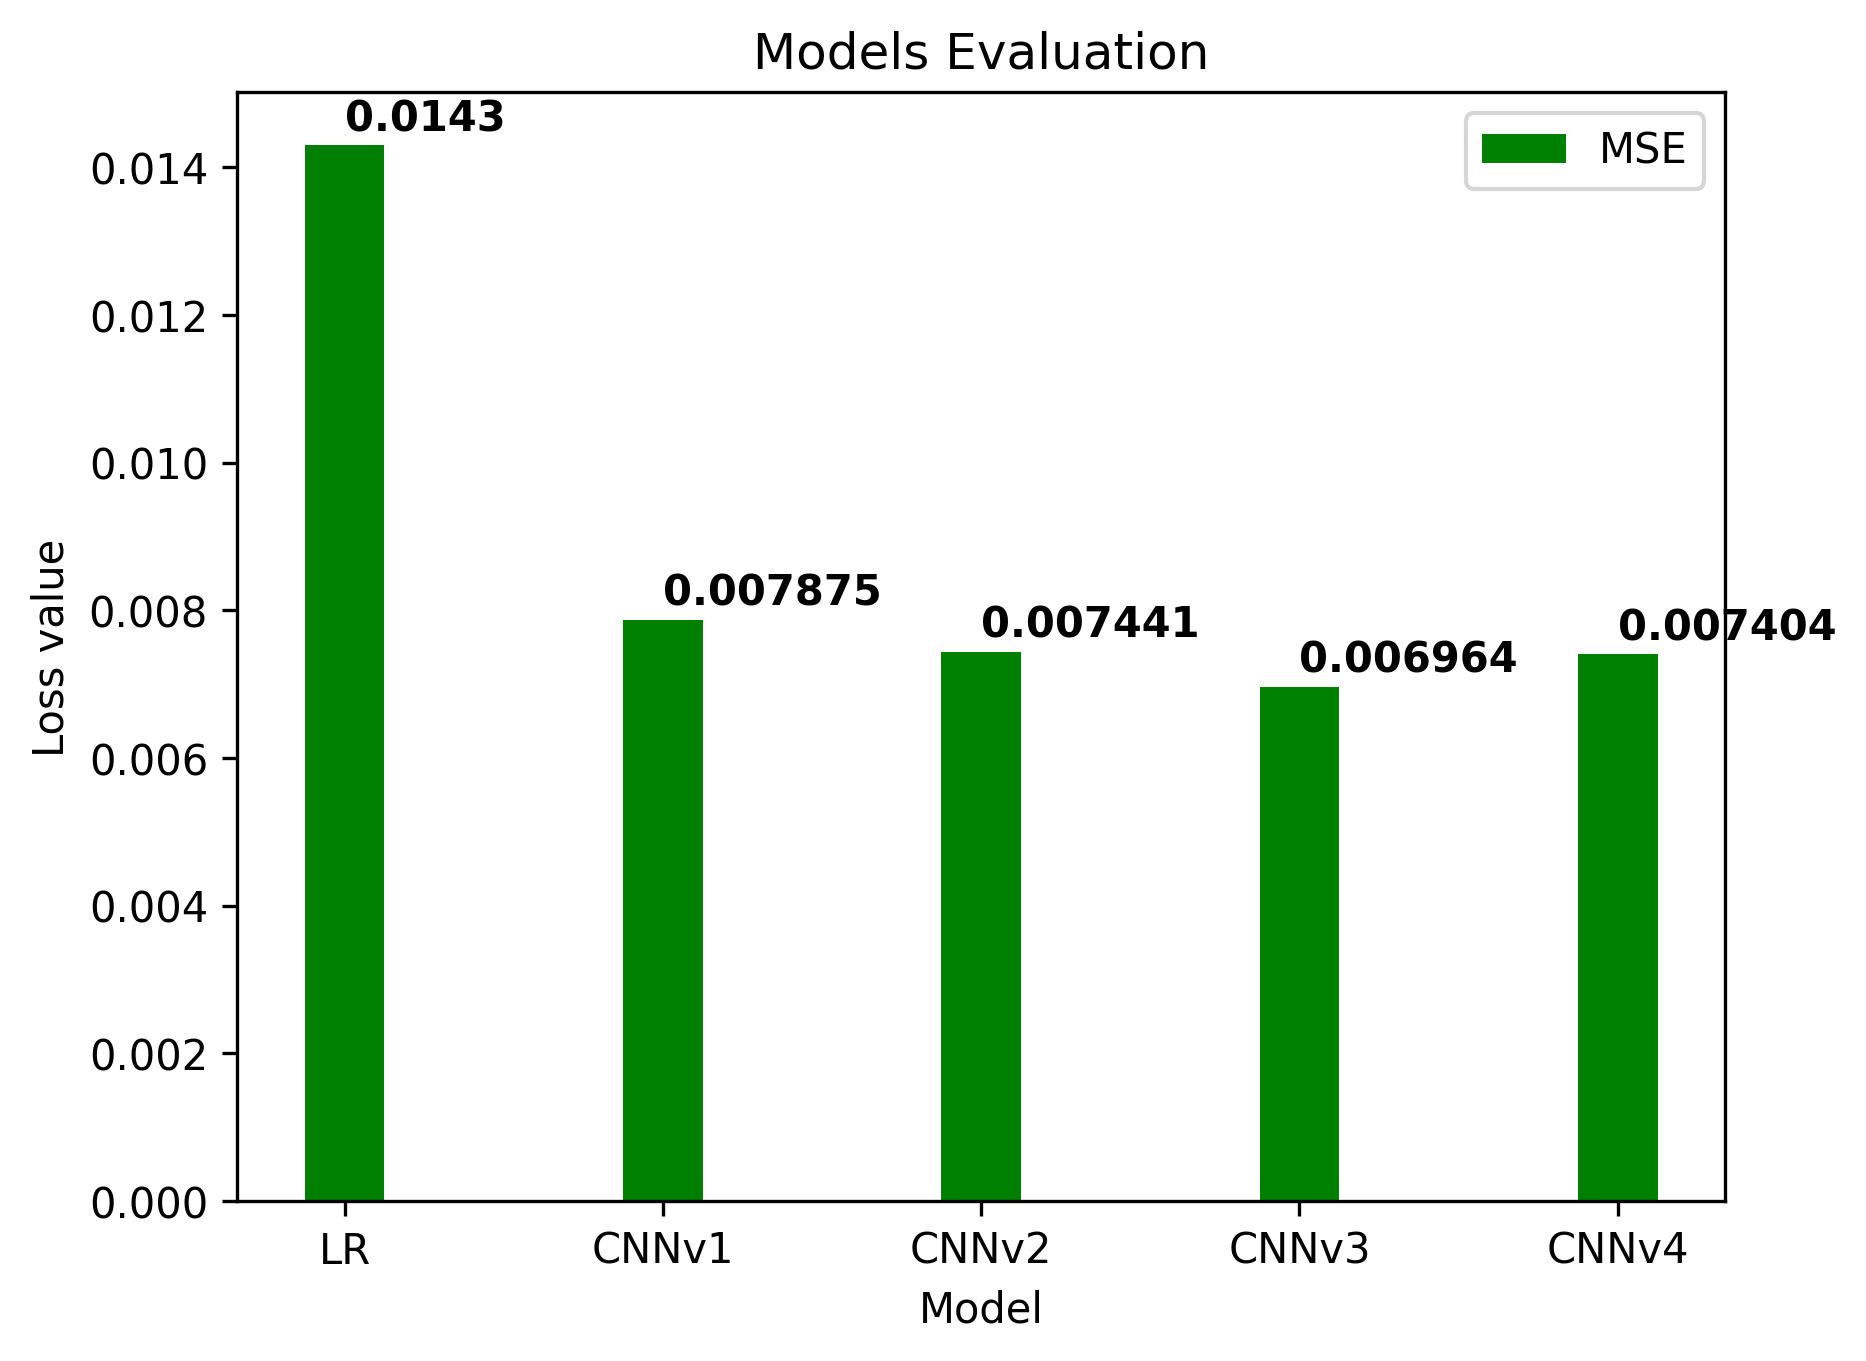
\includegraphics[width=\linewidth]{img/one-trial/models_evaluation_one_trial_mse.png}
    \caption{Models evaluation on MSE.}
  \end{subfigure}
  \\
  \begin{subfigure}[t]{0.45\textwidth}
    \centering
    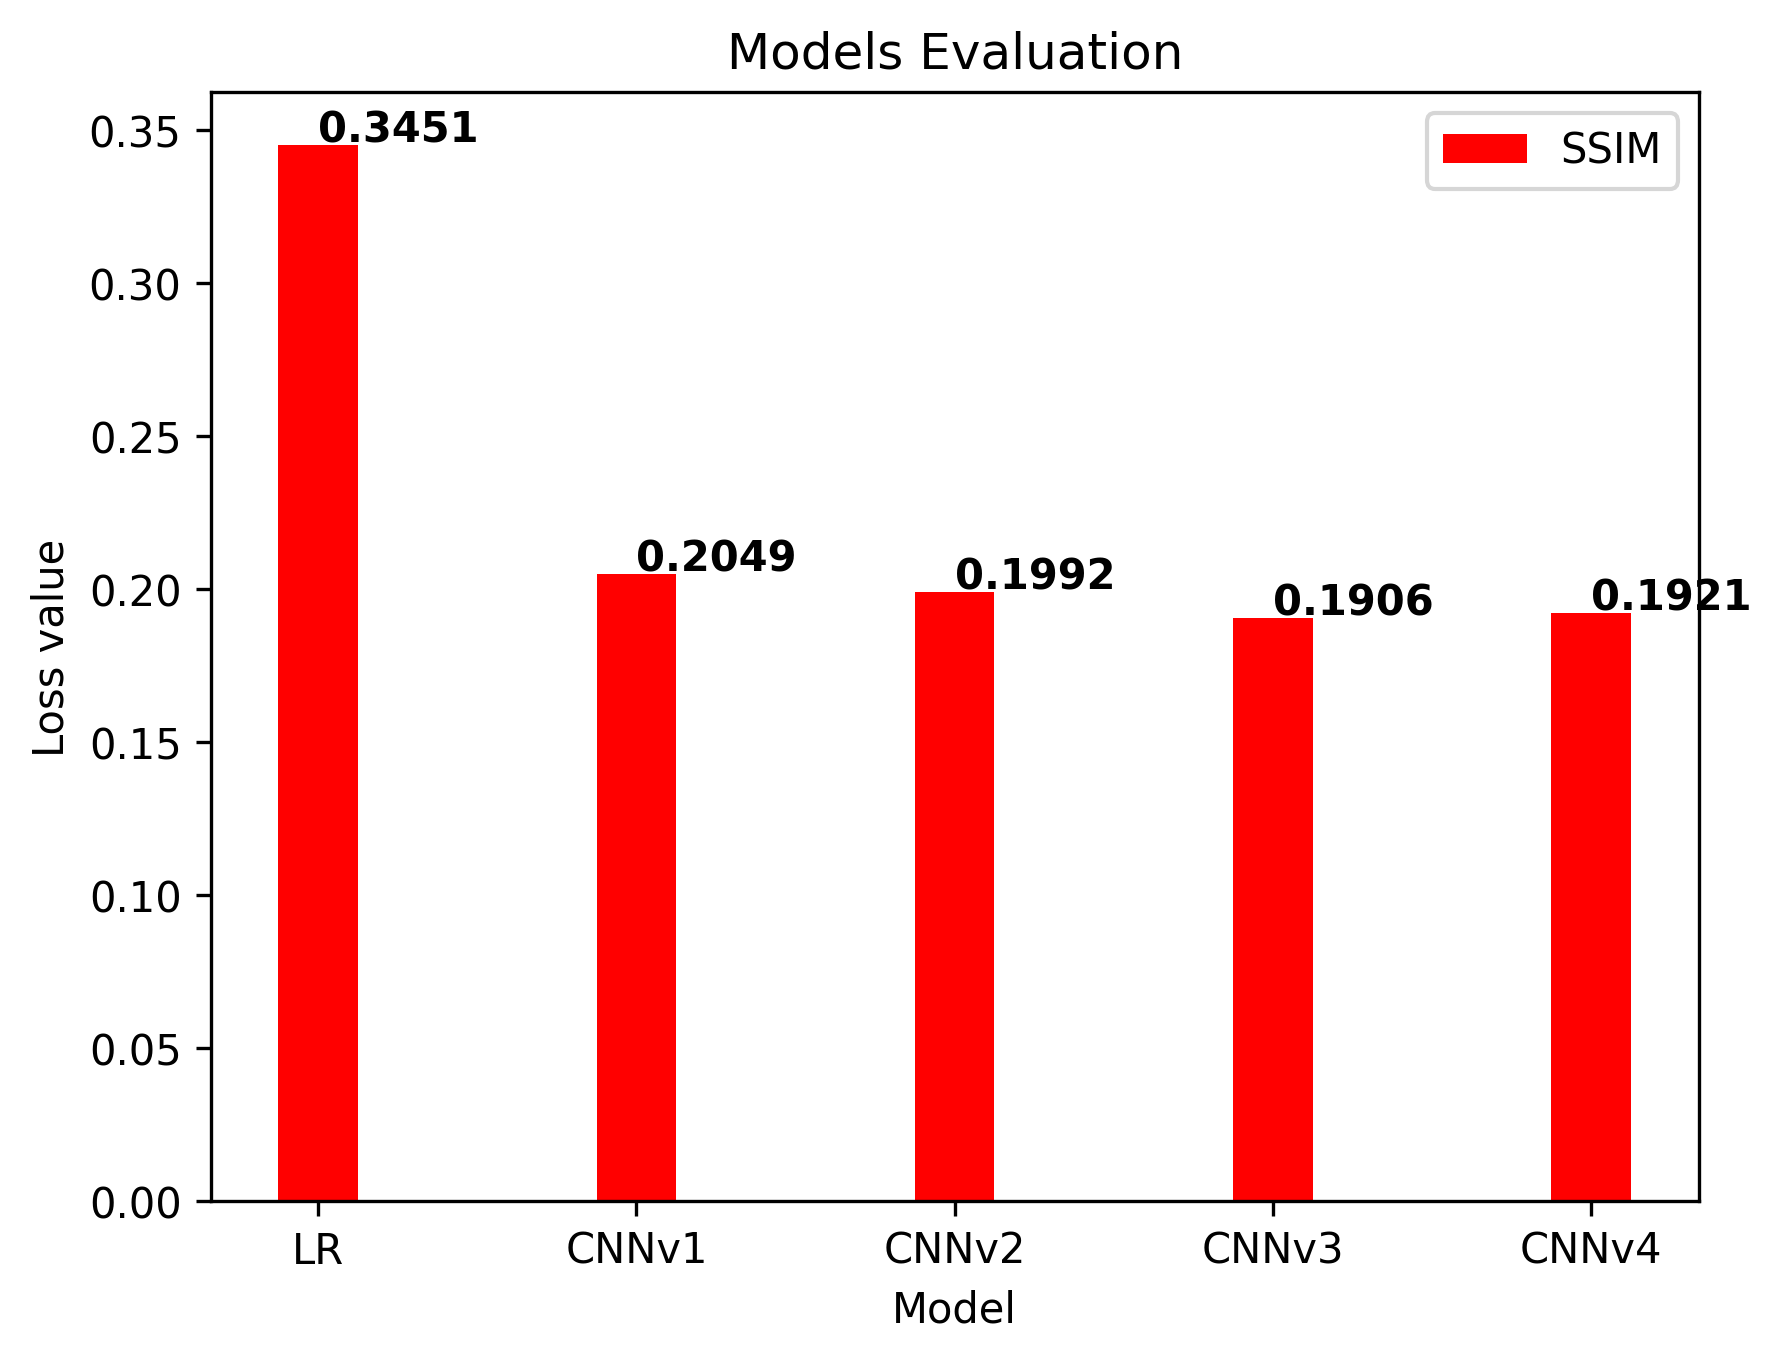
\includegraphics[width=\linewidth]{img/one-trial/models_evaluation_one_trial_ssim.png}
    \caption{Models evaluation on SSIM.}
  \end{subfigure}
  \begin{subfigure}[t]{0.45\textwidth}
    \centering
    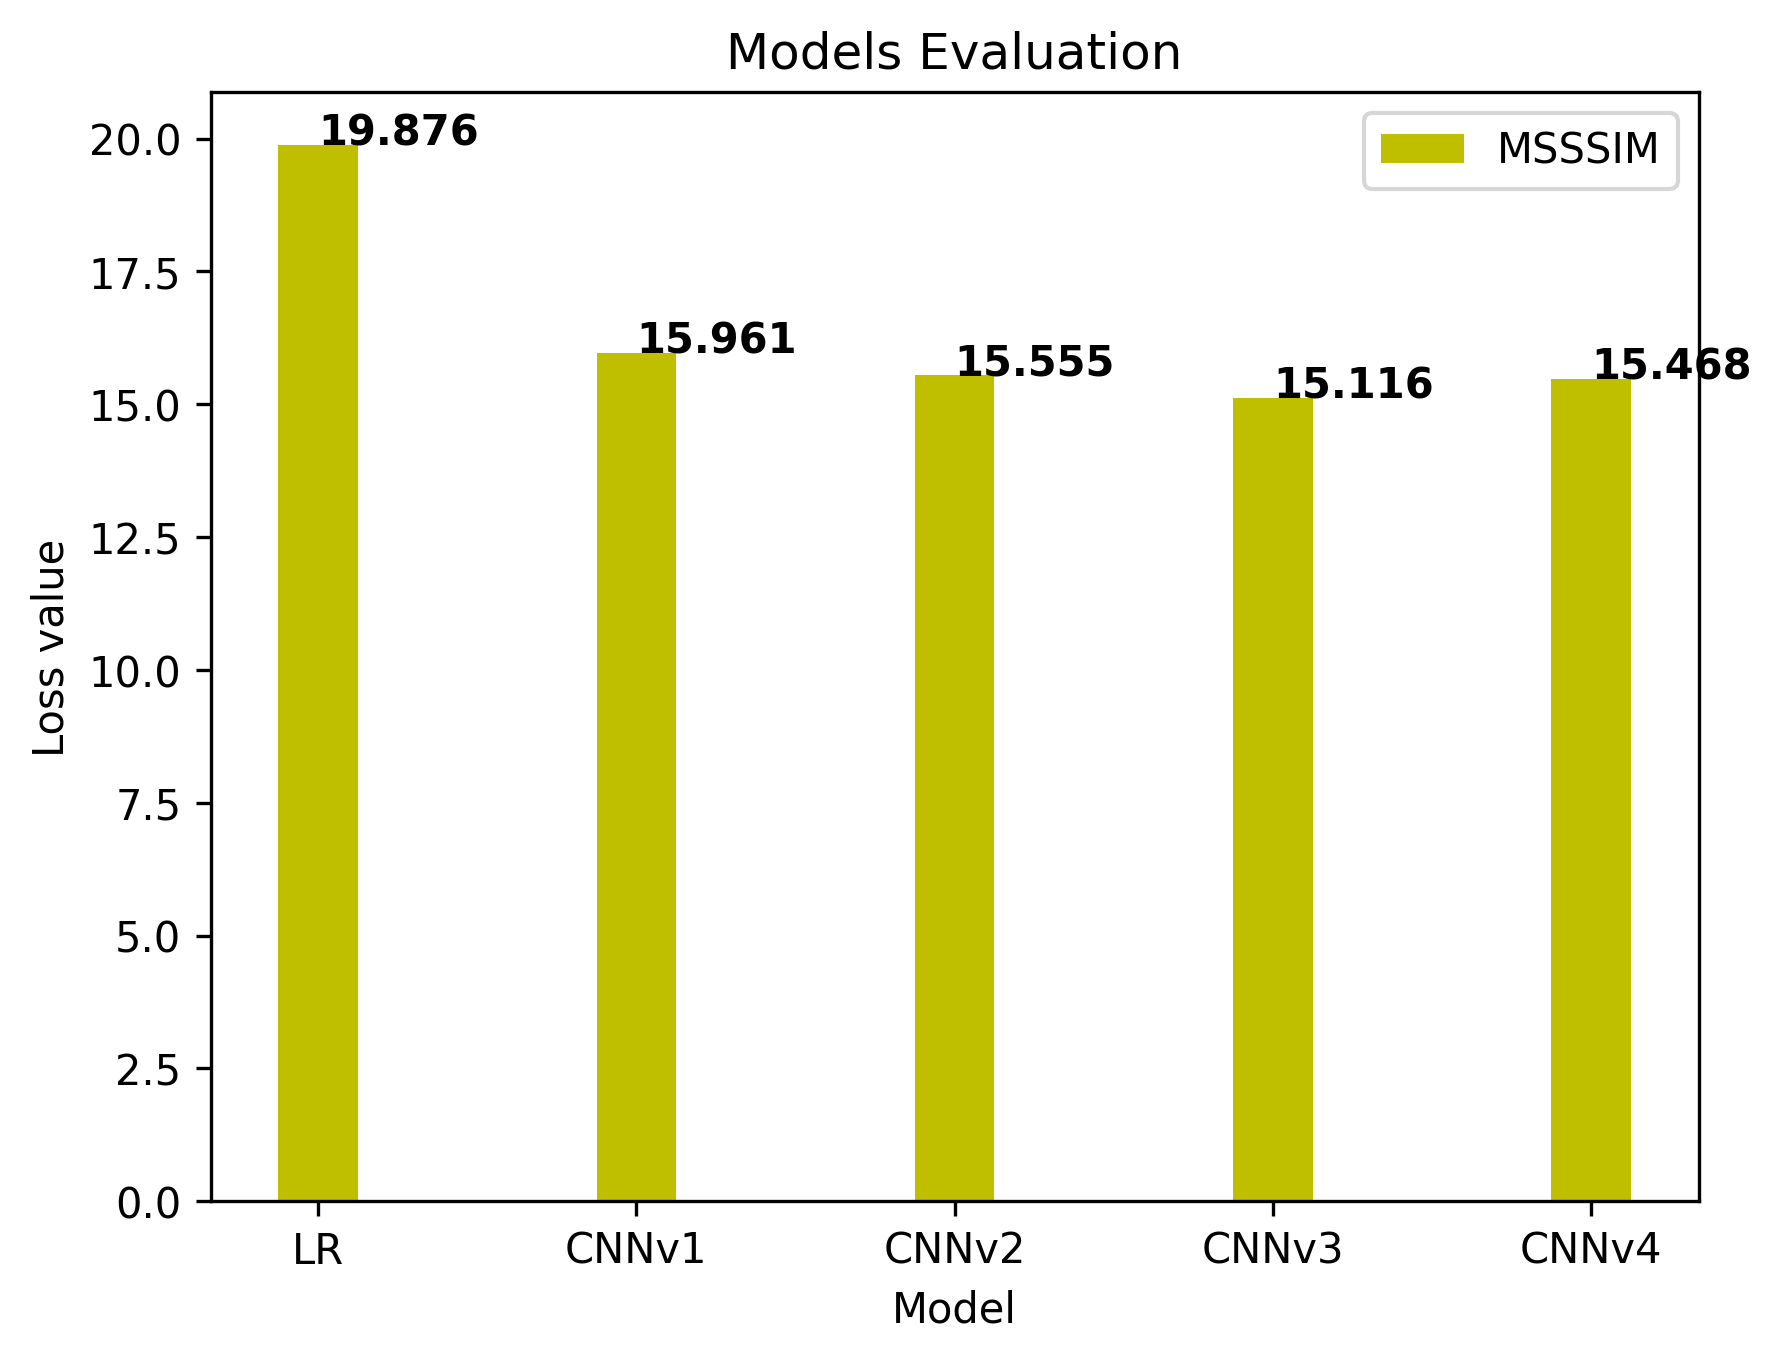
\includegraphics[width=\linewidth]{img/one-trial/models_evaluation_one_trial_msssim.png}
    \caption{Models evaluation on MSSSIM.}
  \end{subfigure}
\caption{Comparison of multiple models on the same (one-trial) dataset using different loss metrics.}
\label{img:experiments:one-trial:comparison}
\end{figure}

On the picture~\ref{img:experiments:one-trial:comparison}, we can see the results separately for $L_1$, MSE, SSIM, and MSSSIM losses. It is clear, that the linear regression model is now the worst, as all the losses are highest for it. On the other hand, we can see that the CNN model's performance is quite similar. The best one of them is model CNNv3, which is slightly better than CNNv4, then we have CNNv2 and CNNv1 is the worst of the CNN models by all four metrics.

\begin{figure}[H]\centering

  \begin{subfigure}[t]{0.15\textwidth}
    \centering
    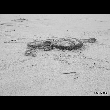
\includegraphics[width=\linewidth]{img/one-trial/stimulus_1.png}
    % \caption{Stim. 1}
  \end{subfigure}
  \begin{subfigure}[t]{0.15\textwidth}
    \centering
    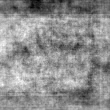
\includegraphics[width=\linewidth]{img/one-trial/prediction_1_lr.png}
    % \caption{LR}
  \end{subfigure}
  \begin{subfigure}[t]{0.15\textwidth}
    \centering
    
\includegraphics[width=\linewidth]{img/one-trial/prediction_1_cnnv1.png}
    % \caption{CNNv1}
  \end{subfigure}
  \begin{subfigure}[t]{0.15\textwidth}
    \centering
    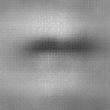
\includegraphics[width=\linewidth]{img/one-trial/prediction_1_cnnv2.png}
    % \caption{CNNv2}
  \end{subfigure}
  \begin{subfigure}[t]{0.15\textwidth}
    \centering
    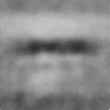
\includegraphics[width=\linewidth]{img/one-trial/prediction_1_cnnv3.png}
    % \caption{CNNv3}
  \end{subfigure}
  \begin{subfigure}[t]{0.15\textwidth}
    \centering
    
\includegraphics[width=\linewidth]{img/one-trial/prediction_1_cnnv4.png}
    % \caption{CNNv4}
  \end{subfigure}
  \\
    \vspace{0.1cm}
  
  \begin{subfigure}[t]{0.15\textwidth}
    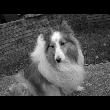
\includegraphics[width=\linewidth]{img/one-trial/stimulus_2.png}
    % \caption{Stim. 2}
  \end{subfigure}
  \begin{subfigure}[t]{0.15\textwidth}
    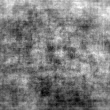
\includegraphics[width=\linewidth]{img/one-trial/prediction_2_lr.png}
    % \caption{LR}
  \end{subfigure}
  \begin{subfigure}[t]{0.15\textwidth}
    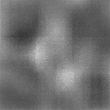
\includegraphics[width=\linewidth]{img/one-trial/prediction_2_cnnv1.png}
    % \caption{CNNv1}
  \end{subfigure}
  \begin{subfigure}[t]{0.15\textwidth}
    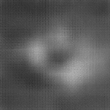
\includegraphics[width=\linewidth]{img/one-trial/prediction_2_cnnv2.png}
    % \caption{CNNv2}
  \end{subfigure}
  \begin{subfigure}[t]{0.15\textwidth}
    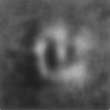
\includegraphics[width=\linewidth]{img/one-trial/prediction_2_cnnv3.png}
    % \caption{CNNv3}
  \end{subfigure}
  \begin{subfigure}[t]{0.15\textwidth}
    
\includegraphics[width=\linewidth]{img/one-trial/prediction_2_cnnv4.png}
    % \caption{CNNv4}
  \end{subfigure}
  \\
    \vspace{0.1cm}
  
  \begin{subfigure}[t]{0.15\textwidth}
    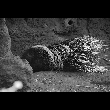
\includegraphics[width=\linewidth]{img/one-trial/stimulus_3.png}
    % \caption{Stim. 3}
  \end{subfigure}
  \begin{subfigure}[t]{0.15\textwidth}
    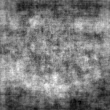
\includegraphics[width=\linewidth]{img/one-trial/prediction_3_lr.png}
    % \caption{LR}
  \end{subfigure}
  \begin{subfigure}[t]{0.15\textwidth}
    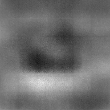
\includegraphics[width=\linewidth]{img/one-trial/prediction_3_cnnv1.png}
    % \caption{CNNv1}
  \end{subfigure}
  \begin{subfigure}[t]{0.15\textwidth}
    
\includegraphics[width=\linewidth]{img/one-trial/prediction_3_cnnv2.png}
    % \caption{CNNv2}
  \end{subfigure}
  \begin{subfigure}[t]{0.15\textwidth}
    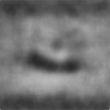
\includegraphics[width=\linewidth]{img/one-trial/prediction_3_cnnv3.png}
    % \caption{CNNv3}
  \end{subfigure}
  \begin{subfigure}[t]{0.15\textwidth}
    
\includegraphics[width=\linewidth]{img/one-trial/prediction_3_cnnv4.png}
    % \caption{CNNv4}
  \end{subfigure}
  \\
    \vspace{0.1cm}
  
  \begin{subfigure}[t]{0.15\textwidth}
    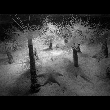
\includegraphics[width=\linewidth]{img/one-trial/stimulus_4.png}
    \caption{Stimuli}
  \end{subfigure}
  \begin{subfigure}[t]{0.15\textwidth}
    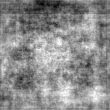
\includegraphics[width=\linewidth]{img/one-trial/prediction_4_lr.png}
    \caption{LR}
  \end{subfigure}
  \begin{subfigure}[t]{0.15\textwidth}
    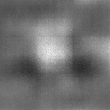
\includegraphics[width=\linewidth]{img/one-trial/prediction_4_cnnv1.png}
    \caption{CNNv1}
  \end{subfigure}
  \begin{subfigure}[t]{0.15\textwidth}
    \includegraphics[width=\linewidth]{img/one-trial/prediction_4_cnnv2.png}
    \caption{CNNv2}
  \end{subfigure}
  \begin{subfigure}[t]{0.15\textwidth}
    \includegraphics[width=\linewidth]{img/one-trial/prediction_4_cnnv3.png}
    \caption{CNNv3}
  \end{subfigure}
  \begin{subfigure}[t]{0.15\textwidth}
    \includegraphics[width=\linewidth]{img/one-trial/prediction_4_cnnv4.png}
    \caption{CNNv4}
  \end{subfigure}
  
\caption{Visual comparison of multiple models on the same cortical activity samples. Each row corresponds to one sample. The first column contains the stimuli targets, each column shows images generated by a different model.}
\label{img:experiments:one-trial:comparison-outputs}
\end{figure}

To better understand the difference in the predictions, we also provide sample outputs for four different cortical activity inputs from the testing part of the dataset~\ref{img:experiments:one-trial:comparison-outputs}. The outputs of the linear regression model look very noisy. The CNNv3 gives results that are convincing both in the loss metrics and also when we compare them visually.

From now on, we use only the best model (CNNv3) to perform the rest of the experiments, which use only one model.


% **************************************************
\subsection{Intermediate Image}
\label{experiments:one-trial:intermediate-image}
Two of our implemented architectures use intermediate images inside the network, namely CNNv3~\ref{methods:models:CNNv3} and CNNv4~\ref{methods:models:CNNv4}. The CNNv3 uses a stack of transposed convolutional layers on top of the intermediate image to produce the output image. CNNv4 instead uses an encoder-decoder type of network to denoise the intermediate image~\citep{zhang2020reconstruction}. We show the intermediate images together with stimuli and output images in the figure~\ref{img:experiments:one-trial:intermediate-image}.


\begin{figure}[H]\centering
  \setcounter{subfigure}{0}
  \begin{subfigure}[t]{0.13\textwidth}
    \centering
    \includegraphics[width=\linewidth]{img/one-trial/stimulus_1.png}
    % \caption{Stim. 1}
  \end{subfigure}
  \begin{subfigure}[t]{0.13\textwidth}
    \centering
    \includegraphics[width=\linewidth]{img/one-trial/intermediate-cnnv3/intermediate_0.png}
    % \caption{CNNv3}
  \end{subfigure}
  \begin{subfigure}[t]{0.13\textwidth}
    \centering
    \includegraphics[width=\linewidth]{img/one-trial/intermediate-cnnv3/prediction_0.png}
    % \caption{CNNv3}
  \end{subfigure}
  \begin{subfigure}[t]{0.13\textwidth}
    \centering
    \includegraphics[width=\linewidth]{img/one-trial/intermediate-cnnv4/intermediate_0.png}
    % \caption{CNNv4}
  \end{subfigure}
  \begin{subfigure}[t]{0.13\textwidth}
    \centering
    \includegraphics[width=\linewidth]{img/one-trial/intermediate-cnnv4/prediction_0.png}
    % \caption{CNNv4}
  \end{subfigure}
  \\
    \vspace{0.1cm}
  
  \setcounter{subfigure}{0}
  \begin{subfigure}[t]{0.13\textwidth}
    \centering
    \includegraphics[width=\linewidth]{img/one-trial/stimulus_2.png}
    % \caption{Stim. 1}
  \end{subfigure}
  \begin{subfigure}[t]{0.13\textwidth}
    \centering
    \includegraphics[width=\linewidth]{img/one-trial/intermediate-cnnv3/intermediate_1.png}
    % \caption{CNNv3}
  \end{subfigure}
  \begin{subfigure}[t]{0.13\textwidth}
    \centering
    \includegraphics[width=\linewidth]{img/one-trial/intermediate-cnnv3/prediction_1.png}
    % \caption{CNNv3}
  \end{subfigure}
  \begin{subfigure}[t]{0.13\textwidth}
    \centering
    \includegraphics[width=\linewidth]{img/one-trial/intermediate-cnnv4/intermediate_1.png}
    % \caption{CNNv4}
  \end{subfigure}
  \begin{subfigure}[t]{0.13\textwidth}
    \centering
    \includegraphics[width=\linewidth]{img/one-trial/intermediate-cnnv4/prediction_1.png}
    % \caption{CNNv4}
  \end{subfigure}
  \\
    \vspace{0.1cm}
  
  \setcounter{subfigure}{0}
  \begin{subfigure}[t]{0.13\textwidth}
    \centering
    \includegraphics[width=\linewidth]{img/one-trial/stimulus_3.png}
    % \caption{Stim. 1}
  \end{subfigure}
  \begin{subfigure}[t]{0.13\textwidth}
    \centering
    \includegraphics[width=\linewidth]{img/one-trial/intermediate-cnnv3/intermediate_2.png}
    % \caption{CNNv3}
  \end{subfigure}
  \begin{subfigure}[t]{0.13\textwidth}
    \centering
    \includegraphics[width=\linewidth]{img/one-trial/intermediate-cnnv3/prediction_2.png}
    % \caption{CNNv3}
  \end{subfigure}
  \begin{subfigure}[t]{0.13\textwidth}
    \centering
    \includegraphics[width=\linewidth]{img/one-trial/intermediate-cnnv4/intermediate_2.png}
    % \caption{CNNv4}
  \end{subfigure}
  \begin{subfigure}[t]{0.13\textwidth}
    \centering
    \includegraphics[width=\linewidth]{img/one-trial/intermediate-cnnv4/prediction_2.png}
    % \caption{CNNv4}
  \end{subfigure}
  \\
    \vspace{0.1cm}
  
  \setcounter{subfigure}{0}
  \begin{subfigure}[t]{0.13\textwidth}
    \centering
    \includegraphics[width=\linewidth]{img/one-trial/stimulus_4.png}
    \caption{Stimuli}
  \end{subfigure}
  \begin{subfigure}[t]{0.13\textwidth}
    \centering
    \includegraphics[width=\linewidth]{img/one-trial/intermediate-cnnv3/intermediate_3.png}
    \caption{CNNv3}
  \end{subfigure}
  \begin{subfigure}[t]{0.13\textwidth}
    \centering
    \includegraphics[width=\linewidth]{img/one-trial/intermediate-cnnv3/prediction_3.png}
    \caption{CNNv3}
  \end{subfigure}
  \begin{subfigure}[t]{0.13\textwidth}
    \centering
    \includegraphics[width=\linewidth]{img/one-trial/intermediate-cnnv4/intermediate_3.png}
    \caption{CNNv4}
  \end{subfigure}
  \begin{subfigure}[t]{0.13\textwidth}
    \centering
    \includegraphics[width=\linewidth]{img/one-trial/intermediate-cnnv4/prediction_3.png}
    \caption{CNNv4}
  \end{subfigure}
  
\caption{Table of images for visual comparison of stimuli images (first column), intermediate images (columns b and d), and the actual output of the models (columns c and e). Each row represents a different sample, columns b and c are generated by model CNNv3, and columns d and e by model CNNv4.}
\label{img:experiments:one-trial:intermediate-image}
\end{figure}

Based on the intermediate images, we conclude that the model CNNv3 is producing an image that is much closer to the one which is then generated as an output, although it contains much more noise than the output image. The model CNNv4 is generating an intermediate image, which looks very noisy, there is no visual similarity with the output and the idea to use the encoder-decoder architecture to enhance the intermediate image is therefore questionable.


% **************************************************
\subsection{Finding Best Loss Function}
\label{experiments:one-trial:finding-best-loss}
We used the CNNv3 model and trained it using all the loss functions defined in~\ref{methods:losses}. The results are on plots~\ref{img:experiments:one-trial:finding-best-loss-bars}.

\begin{figure}[H]\centering
  \begin{subfigure}[t]{0.45\textwidth}
    \centering
    \includegraphics[width=\linewidth]{img/one-trial/model_loss_one_trial_l1.png}
    \caption{Models evaluation on $L_1$.}
  \end{subfigure}
  \begin{subfigure}[t]{0.45\textwidth}
    \centering
    \includegraphics[width=\linewidth]{img/one-trial/model_loss_one_trial_mse.png}
    \caption{Models evaluation on MSE.}
  \end{subfigure}
  \\
  \begin{subfigure}[t]{0.45\textwidth}
    \centering
    \includegraphics[width=\linewidth]{img/one-trial/model_loss_one_trial_ssim.png}
    \caption{Models evaluation on SSIM.}
  \end{subfigure}
  \begin{subfigure}[t]{0.45\textwidth}
    \centering
    \includegraphics[width=\linewidth]{img/one-trial/model_loss_one_trial_msssim.png}
    \caption{Models evaluation on MSSSIM.}
  \end{subfigure}
\caption{Comparison showing how final testing/validation loss depends on different training losses.}
\label{img:experiments:one-trial:finding-best-loss-bars}
\end{figure}

Interestingly we found that no matter which of the four main loss metrics is used as the target one, we get the best results when we train using the MSSSIM loss. We also show how the results differ when we use different training losses visually on picture~\ref{img:experiments:one-trial:finding-best-loss-outputs}.

\begin{figure}[H]\centering
  \setcounter{subfigure}{0}
  \begin{subfigure}[t]{0.13\textwidth}
    \centering
    \includegraphics[width=\linewidth]{img/one-trial/stimulus_1.png}
    % \caption{Stim. 1}
  \end{subfigure}
  \begin{subfigure}[t]{0.13\textwidth}
    \centering
    \includegraphics[width=\linewidth]{img/one-trial/prediction_1_l1.png}
    % \caption{L1}
  \end{subfigure}
  \begin{subfigure}[t]{0.13\textwidth}
    \centering
    \includegraphics[width=\linewidth]{img/one-trial/prediction_1_mse.png}
    % \caption{MSE}
  \end{subfigure}
  \begin{subfigure}[t]{0.13\textwidth}
    \centering
    \includegraphics[width=\linewidth]{img/one-trial/prediction_1_ssim.png}
    % \caption{SSIM}
  \end{subfigure}
  \begin{subfigure}[t]{0.13\textwidth}
    \centering
    \includegraphics[width=\linewidth]{img/one-trial/prediction_1_msssim.png}
    % \caption{MSSSIM}
  \end{subfigure}
  \begin{subfigure}[t]{0.13\textwidth}
    \centering
    \includegraphics[width=\linewidth]{img/one-trial/prediction_1_mix.png}
    % \caption{MIX}
  \end{subfigure}
  \begin{subfigure}[t]{0.13\textwidth}
    \centering
    \includegraphics[width=\linewidth]{img/one-trial/prediction_1_adversarial.png}
    % \caption{Adversarial}
  \end{subfigure}
  \\
    \vspace{0.1cm}
  
  \setcounter{subfigure}{0}
  \begin{subfigure}[t]{0.13\textwidth}
    \centering
    \includegraphics[width=\linewidth]{img/one-trial/stimulus_2.png}
    % \caption{Stim. 1}
  \end{subfigure}
  \begin{subfigure}[t]{0.13\textwidth}
    \centering
    \includegraphics[width=\linewidth]{img/one-trial/prediction_2_l1.png}
    % \caption{L1}
  \end{subfigure}
  \begin{subfigure}[t]{0.13\textwidth}
    \centering
    \includegraphics[width=\linewidth]{img/one-trial/prediction_2_mse.png}
    % \caption{MSE}
  \end{subfigure}
  \begin{subfigure}[t]{0.13\textwidth}
    \centering
    \includegraphics[width=\linewidth]{img/one-trial/prediction_2_ssim.png}
    % \caption{SSIM}
  \end{subfigure}
  \begin{subfigure}[t]{0.13\textwidth}
    \centering
    \includegraphics[width=\linewidth]{img/one-trial/prediction_2_msssim.png}
    % \caption{MSSSIM}
  \end{subfigure}
  \begin{subfigure}[t]{0.13\textwidth}
    \centering
    \includegraphics[width=\linewidth]{img/one-trial/prediction_2_mix.png}
    % \caption{MIX}
  \end{subfigure}
  \begin{subfigure}[t]{0.13\textwidth}
    \centering
    \includegraphics[width=\linewidth]{img/one-trial/prediction_2_adversarial.png}
    % \caption{Adversarial}
  \end{subfigure}
  \\
    \vspace{0.1cm}
  
  \setcounter{subfigure}{0}
  \begin{subfigure}[t]{0.13\textwidth}
    \centering
    \includegraphics[width=\linewidth]{img/one-trial/stimulus_3.png}
    % \caption{Stim. 1}
  \end{subfigure}
  \begin{subfigure}[t]{0.13\textwidth}
    \centering
    \includegraphics[width=\linewidth]{img/one-trial/prediction_3_l1.png}
    % \caption{L1}
  \end{subfigure}
  \begin{subfigure}[t]{0.13\textwidth}
    \centering
    \includegraphics[width=\linewidth]{img/one-trial/prediction_3_mse.png}
    % \caption{MSE}
  \end{subfigure}
  \begin{subfigure}[t]{0.13\textwidth}
    \centering
    \includegraphics[width=\linewidth]{img/one-trial/prediction_3_ssim.png}
    % \caption{SSIM}
  \end{subfigure}
  \begin{subfigure}[t]{0.13\textwidth}
    \centering
    \includegraphics[width=\linewidth]{img/one-trial/prediction_3_msssim.png}
    % \caption{MSSSIM}
  \end{subfigure}
  \begin{subfigure}[t]{0.13\textwidth}
    \centering
    \includegraphics[width=\linewidth]{img/one-trial/prediction_3_mix.png}
    % \caption{MIX}
  \end{subfigure}
  \begin{subfigure}[t]{0.13\textwidth}
    \centering
    \includegraphics[width=\linewidth]{img/one-trial/prediction_3_adversarial.png}
    % \caption{Adversarial}
  \end{subfigure}
  \\
    \vspace{0.1cm}
  
  \setcounter{subfigure}{0}
  \begin{subfigure}[t]{0.13\textwidth}
    \centering
    \includegraphics[width=\linewidth]{img/one-trial/stimulus_4.png}
    \caption{Stimuli}
  \end{subfigure}
  \begin{subfigure}[t]{0.13\textwidth}
    \centering
    \includegraphics[width=\linewidth]{img/one-trial/prediction_4_l1.png}
    \caption{L1}
  \end{subfigure}
  \begin{subfigure}[t]{0.13\textwidth}
    \centering
    \includegraphics[width=\linewidth]{img/one-trial/prediction_4_mse.png}
    \caption{MSE}
  \end{subfigure}
  \begin{subfigure}[t]{0.13\textwidth}
    \centering
    \includegraphics[width=\linewidth]{img/one-trial/prediction_4_ssim.png}
    \caption{SSIM}
  \end{subfigure}
  \begin{subfigure}[t]{0.13\textwidth}
    \centering
    \includegraphics[width=\linewidth]{img/one-trial/prediction_4_msssim.png}
    \caption{MSSSIM}
  \end{subfigure}
  \begin{subfigure}[t]{0.13\textwidth}
    \centering
    \includegraphics[width=\linewidth]{img/one-trial/prediction_4_mix.png}
    \caption{MIX}
  \end{subfigure}
  \begin{subfigure}[t]{0.13\textwidth}
    \centering
    \includegraphics[width=\linewidth]{img/one-trial/prediction_4_adversarial.png}
    \caption{Discriminator}
  \end{subfigure}
  
\caption{Visual comparison of multiple models, each trained with a different loss function. Each row corresponds to one sample. The first column contains the stimuli targets, other columns show images generated by different models.}
\label{img:experiments:one-trial:finding-best-loss-outputs}
\end{figure}

When compared visually, it corresponds also to the low value of loss metrics, that the model trained with MSSSIM loss is one of the best ones. The results of the discriminator loss also look like they can depict higher frequencies and contrast better, but this model does not look so well when measured by the loss metrics. We can therefore conclude, that the subjective human visual comparison can sometimes differ from the mathematical-based loss metrics.

% **************************************************
\subsection{Evaluating Dataset Size}
\label{experiments:one-trial:number-of-samples}
To inspect how important is to have enough samples when training the models, we did a sweep on the dataset size. For the given number of samples $n \in \mathbb{N}$, we selected only the first part of the training samples so that only the first $n$ samples were used. We trained only on those, selected the best model state based on the validation part, and evaluated on the same testing part. In other words, only the training set size was variable in each run.

The results are on image~\ref{img:experiments:one-trial:number-of-samples}. We observed that with more samples, the model was able to perform better in terms of the $L_1$ loss. We also observed some noise in the measurements (the values are not always decreasing monotonically) which was expected, as the training of the CNN models is not deterministic.

\begin{figure}[H]\centering
\includegraphics[width=140mm]{img/one-trial/dataset_size_one_trial.png}
\caption{Dependency of model $L_1$ loss on the size of the dataset in several training samples.}
\label{img:experiments:one-trial:number-of-samples}
\end{figure}


% **************************************************
\subsection{Exploring Number of Input Neurons}
\label{experiments:one-trial:number-of-inputs}
To show the importance of the cortical activity neurons, we did another sweep, where the variable was the number of neurons from the cortical activity, which the model was able to use. For each number of neurons, the neurons were selected randomly, the model was trained on the whole training part, the best model was selected using the validation set, and the results on the testing part were used to plot the values in this graph.

The results are on image~\ref{img:experiments:one-trial:number-of-inputs}. The maximum number of neurons is $60000$, which produces the best $L_1$ value. We can again see a dependency, which shows us that using more neurons helps the model to find a better solution.

\begin{figure}[H]\centering
\includegraphics[width=140mm]{img/one-trial/response_size_one_trial.png}
\caption{Dependency of $L_1$ loss on the number of used cortical activity neurons for the training.}
\label{img:experiments:one-trial:number-of-inputs}
\end{figure}


% **************************************************
\subsection{Exploring Neuron Population Importance}
\label{experiments:one-trial:population-importance}
The number of all neurons from the cortical activity is 60000. In all of our models, the number of parameters was mainly high in the first layers, as the input vector dimensionality reduction was done by fully connected, or convolutional layers. We are provided with information for each neuron, whether it is coming from L4 or L2/3 layer and also whether it is an excitatory or inhibitory one. In this experiment, we use this information to evaluate the performance of separate groups of neurons. For each group of neurons, we select a random subsection and use only that subsection for the training, validation, and testing.

The first plot~\ref{img:experiments:one-trial:population-importance:all} shows the evaluation, when we use all neurons (red color), only neurons from the L2/3 layer (blue color), and only neurons from the L4 layer (green color). From this plot, it is apparent, that the most informative layer is the L4. By using only this layer, we can train a model, which performs at least the same (in our case even a little bit better ($L_1=0.06621$ using only 23838 neurons)) in terms of $L_1$ loss, than the best model, which uses all of the neurons ($L_1=0.06655$ using 60000 neurons). The results for the L4 layer and usage of all neurons are much closer than the L2/3 layer, which produces models of $L_1$ loss higher by approximately $0.01$. That makes it much less informative than the L4 layer.

\begin{figure}[H]\centering
\includegraphics[width=140mm]{img/one-trial/responses_size_groups_one_trial.png}
\caption{Dependency of $L_1$ loss on the number of used cortical activity neurons for the training for different neuron population groups, each colored in a different hue.}
\label{img:experiments:one-trial:population-importance:all}
\end{figure}

The result of the previous experiment on the L4 layer encouraged us to try to separate the neurons of L4 by their function (excitatory, inhibitory). The number of excitatory neurons is 24000, and we have 6000 inhibitory neurons in the L4 layer. The results are present in plot~\ref{img:experiments:one-trial:population-importance:L4}. We have the whole population of neurons and the whole L4 population colored as in the previous plot by red and green colors. The excitatory population of neurons is colored by yellow and the inhibitory population by purple colors. From this plot, we can see even more interesting results. By using only the inhibitory neurons of L4 (6000), we are able to train models, which perform much better than models which use other groups of neurons.

\begin{figure}[H]\centering
\includegraphics[width=140mm]{img/one-trial/responses_size_l4_groups_one_trial.png}
% \includegraphics[width=140mm]{img/one-trial/responses_size_l4_groups_one_trial_noall.png}
\caption{Dependency of $L_1$ loss on the number of used cortical activity neurons for the training for all neurons, and also separately excitatory and inhibitory neurons from L4. %\todo{which of the two plots is better to use?}
}
\label{img:experiments:one-trial:population-importance:L4}
\end{figure}

From this experiment, we conclude, that the most important group of neurons is the L4 inhibitory population, which produces the best model with $L_1=0.06609$ on the testing set.


% % **************************************************
% \subsection{Regularization}
% \label{experiments:one-trial:regularization}

% \todo{using stimulus augmentations, layer dropout, inner fully connected layer size... maybe exclude this whole subsection, the regularization techniques did not improve the accuracy anyway...}



% ==================================================
\section{Losses}
\label{experiments:losses}
To gain a better understanding of how the selected loss functions behave under different perturbations, to evaluate their performance, and understand better their values, we employed several image perturbations. These perturbations were chosen with the aim of generating a diverse set of image variations that can provide insights into the properties of the loss functions. By evaluating the performance of the loss functions on these perturbed images, we can gain a better understanding of their strengths and weaknesses. Furthermore, by visualizing the perturbed images, we can analyze the visual impact of the perturbations on the generated images and determine the quality of the generated images subjectively as human observers. Overall, image perturbations provide a useful tool for evaluating and comparing the performance of different loss functions.

The selected perturbations are:
\begin{itemize}
    \item Gaussian blur with kernel size 65 and sigma 10
    \item Gaussian noise with mean 0 and std 0.1
    \item Value noise, which randomly for each pixel adds or subtracts value 0.07
    \item Intensity shift, which adds 0.07 to all pixels
    \item Image translation, which rolls the image in Y axis by 9 pixels
\end{itemize}

We first used a central crop of 64x64 pixels of the original stimulus image (the reason is that the same crop was used for the evaluation of the models). We applied the perturbation, clip the image to the [0;1] range, and computed the mean loss value of the perturbed and the original stimulus image. The loss values are on top of every single image.

The parameters of perturbations were selected so that the loss value of L1 is close to $0.07$, which is the best $L_1$ loss achieved in the experiments~(\ref{experiments:one-trial:finding-best-model}) on the one-trial dataset~(\ref{dataset:one-trial}).


% **************************************************
\subsection{Perturbed Images}
\label{experiments:losses:L1}
The values for $L_1$ loss should all be close to $0.07$, as the parameters of the perturbations were selected to hold this condition. Note that it is particularly hard to select parameters of the Gaussian blur, as it has only a very low effect on the $L_1$ loss. In other words, all of the following perturbed images are a possible outcome of the generator model when the $L_1$ is of this value.

Visual results together with the $L_1$ loss values for two test images are in the picture~\ref{img:experiments:losses:L1}. The advantage of this loss is the interpretability. If we use value noise of size $v \in \mathbb{R}$, which adds exactly $v$ or $-v$, the $L_1$ will be exactly $v$, as all the pixel values differ by exactly $v$. If we do an intensity shift of all pixel values by $v$, the $L_1$ is again exactly $v$ by definition.

In the image~\ref{img:experiments:losses:L1}, we see that although all images have a similar $L_1$ value, there are visual differences, that would probably lead to human opinion, that the image perturbed with Gaussian blur is the most different from the original image, and the one perturbed with intensity shift is the most similar one.
If we do an image translation, the images will be visually almost identical, but the $L_1$ loss will become high.

\begin{figure}[H]\centering
  \begin{subfigure}[t]{0.15\textwidth}
    \centering
    \includegraphics[width=\linewidth]{img/one-trial/loss_eval/L1/stimulus_0_original_L1.png}
    % \caption{Stim. 1}
  \end{subfigure}
  \begin{subfigure}[t]{0.15\textwidth}
    \centering
    \includegraphics[width=\linewidth]{img/one-trial/loss_eval/L1/stimulus_0_blur_65_10_L1.png}
    % \caption{G. Blur}
  \end{subfigure}
  \begin{subfigure}[t]{0.15\textwidth}
    \centering
    \includegraphics[width=\linewidth]{img/one-trial/loss_eval/L1/stimulus_0_noise_0.1_L1.png}
    % \caption{G. Noise}
  \end{subfigure}
  \begin{subfigure}[t]{0.15\textwidth}
    \centering
    \includegraphics[width=\linewidth]{img/one-trial/loss_eval/L1/stimulus_0_value_noise_0.07_L1.png}
    % \caption{V. Noise}
  \end{subfigure}
  \begin{subfigure}[t]{0.15\textwidth}
    \centering
    \includegraphics[width=\linewidth]{img/one-trial/loss_eval/L1/stimulus_0_value_shift_0.07_L1.png}
    % \caption{Intensity}
  \end{subfigure}
  \begin{subfigure}[t]{0.15\textwidth}
    \centering
    \includegraphics[width=\linewidth]{img/one-trial/loss_eval/L1/stimulus_0_image_shift_x_9_L1.png}
    % \caption{Translation}
  \end{subfigure}
  \\
    \vspace{0.1cm}
    
  \begin{subfigure}[t]{0.15\textwidth}
    \centering
    \includegraphics[width=\linewidth]{img/one-trial/loss_eval/L1/stimulus_1_original_L1.png}
    \caption{Stimuli}
  \end{subfigure}
  \begin{subfigure}[t]{0.15\textwidth}
    \centering
    \includegraphics[width=\linewidth]{img/one-trial/loss_eval/L1/stimulus_1_blur_65_10_L1.png}
    \caption{G. Blur}
  \end{subfigure}
  \begin{subfigure}[t]{0.15\textwidth}
    \centering
    \includegraphics[width=\linewidth]{img/one-trial/loss_eval/L1/stimulus_1_noise_0.1_L1.png}
    \caption{G. Noise}
  \end{subfigure}
  \begin{subfigure}[t]{0.15\textwidth}
    \centering
    \includegraphics[width=\linewidth]{img/one-trial/loss_eval/L1/stimulus_1_value_noise_0.07_L1.png}
    \caption{V. Noise}
  \end{subfigure}
  \begin{subfigure}[t]{0.15\textwidth}
    \centering
    \includegraphics[width=\linewidth]{img/one-trial/loss_eval/L1/stimulus_1_value_shift_0.07_L1.png}
    \caption{Intensity}
  \end{subfigure}
  \begin{subfigure}[t]{0.15\textwidth}
    \centering
    \includegraphics[width=\linewidth]{img/one-trial/loss_eval/L1/stimulus_1_image_shift_x_9_L1.png}
    \caption{Translation}
  \end{subfigure}
\caption{Each row of this figure shows results for a different testing image. The first row contains the original stimuli, the following columns show blurred, noisy, intensity-shifted, and translated original images together with the $L_1$ loss value on top of the images.}
\label{img:experiments:losses:L1}
\end{figure}


%% **************************************************
%\subsection{MSE}
%\label{experiments:losses:MSE}
%\todo{do we need this subsection?}
%We used the same two testing stimuli images and 
%The visual results and MSE loss function values for two testing stimuli and the same augmented images are in the picture. Note that the MSE value was for all these perturbations very low (below 0.01). To better distinguish between the MSE values, see section~\ref{experiments:losses:evaluation-on-dataset}.


%% **************************************************
%\subsection{SSIM}
%\label{experiments:losses:SSIM}


% % **************************************************
% \subsection{MSSSIM}
% \label{experiments:losses:MSSSIM}
% For the computation of MSSSIM loss, we used implementation by Kornia library.\footnote{Available at \url{https://kornia.github.io}.}

% \todo{do we need the images here? maybe it is enough to have them in L1 section}

% \begin{figure}[H]\centering
%   \begin{subfigure}[t]{0.15\textwidth}
%     \centering
%     \includegraphics[width=\linewidth]{img/one-trial/loss_eval/MSSSIM/stimulus_0_original_MSSSIM.png}
%     \caption{Stim. 1}
%   \end{subfigure}
%   \begin{subfigure}[t]{0.15\textwidth}
%     \centering
%     \includegraphics[width=\linewidth]{img/one-trial/loss_eval/MSSSIM/stimulus_0_blur_65_10_MSSSIM.png}
%     \caption{G. Blur}
%   \end{subfigure}
%   \begin{subfigure}[t]{0.15\textwidth}
%     \centering
%     \includegraphics[width=\linewidth]{img/one-trial/loss_eval/MSSSIM/stimulus_0_noise_0.1_MSSSIM.png}
%     \caption{G. Noise}
%   \end{subfigure}
%   \begin{subfigure}[t]{0.15\textwidth}
%     \centering
%     \includegraphics[width=\linewidth]{img/one-trial/loss_eval/MSSSIM/stimulus_0_value_noise_0.07_MSSSIM.png}
%     \caption{V. Noise}
%   \end{subfigure}
%   \begin{subfigure}[t]{0.15\textwidth}
%     \centering
%     \includegraphics[width=\linewidth]{img/one-trial/loss_eval/MSSSIM/stimulus_0_value_shift_0.07_MSSSIM.png}
%     \caption{Intensity}
%   \end{subfigure}
%   \begin{subfigure}[t]{0.15\textwidth}
%     \centering
%     \includegraphics[width=\linewidth]{img/one-trial/loss_eval/MSSSIM/stimulus_0_image_shift_x_9_MSSSIM.png}
%     \caption{Translation}
%   \end{subfigure}
%   \\
%     \vspace{0.5cm}
%   \begin{subfigure}[t]{0.15\textwidth}
%     \centering
%     \includegraphics[width=\linewidth]{img/one-trial/loss_eval/MSSSIM/stimulus_1_original_MSSSIM.png}
%     \caption{Stim. 2}
%   \end{subfigure}
%   \begin{subfigure}[t]{0.15\textwidth}
%     \centering
%     \includegraphics[width=\linewidth]{img/one-trial/loss_eval/MSSSIM/stimulus_1_blur_65_10_MSSSIM.png}
%     \caption{G. Blur}
%   \end{subfigure}
%   \begin{subfigure}[t]{0.15\textwidth}
%     \centering
%     \includegraphics[width=\linewidth]{img/one-trial/loss_eval/MSSSIM/stimulus_1_noise_0.1_MSSSIM.png}
%     \caption{G. Noise}
%   \end{subfigure}
%   \begin{subfigure}[t]{0.15\textwidth}
%     \centering
%     \includegraphics[width=\linewidth]{img/one-trial/loss_eval/MSSSIM/stimulus_1_value_noise_0.07_MSSSIM.png}
%     \caption{V. Noise}
%   \end{subfigure}
%   \begin{subfigure}[t]{0.15\textwidth}
%     \centering
%     \includegraphics[width=\linewidth]{img/one-trial/loss_eval/MSSSIM/stimulus_1_value_shift_0.07_MSSSIM.png}
%     \caption{Intensity}
%   \end{subfigure}
%   \begin{subfigure}[t]{0.15\textwidth}
%     \centering
%     \includegraphics[width=\linewidth]{img/one-trial/loss_eval/MSSSIM/stimulus_1_image_shift_x_9_MSSSIM.png}
%     \caption{Translation}
%   \end{subfigure}
% \caption{\todo{caption}.}
% \label{img:experiments:losses:MSSSIM}
% \end{figure}


% **************************************************
\subsection{Evaluation On Dataset}
\label{experiments:losses:evaluation-on-dataset}
In this experiment, we investigate the influence of each perturbation on the four main basic loss functions used in our thesis. To accomplish this, we use the training part of the ten-trials dataset~(\ref{dataset:ten-trials}) and evaluate all the perturbations on this dataset, which contains $3500$ samples. 
Our goal is to understand how each loss function is affected in different ways by different image perturbations. To achieve this, we calculate the mean loss value for each perturbation and loss function on the entire dataset~(\ref{img:experiments:losses:evaluation-on-dataset:losses}). The results are shown separately for each loss function, with each bar in the plot corresponding to one perturbation.

\begin{figure}[H]\centering
  \begin{subfigure}[t]{0.45\textwidth}
    \centering
    \includegraphics[width=\linewidth]{img/ten-trials/losses/augmentation_L1.png}
    \caption{Models evaluation on $L_1$.}
  \end{subfigure}
  \begin{subfigure}[t]{0.45\textwidth}
    \centering
    \includegraphics[width=\linewidth]{img/ten-trials/losses/augmentation_MSE.png}
    \caption{Models evaluation on MSE.}
  \end{subfigure}
  \\
  \begin{subfigure}[t]{0.45\textwidth}
    \centering
    \includegraphics[width=\linewidth]{img/ten-trials/losses/augmentation_SSIM.png}
    \caption{Models evaluation on SSIM.}
  \end{subfigure}
  \begin{subfigure}[t]{0.45\textwidth}
    \centering
    \includegraphics[width=\linewidth]{img/ten-trials/losses/augmentation_MSSSIM.png}
    \caption{Models evaluation on MSSSIM.}
  \end{subfigure}
\caption{Evaluation of all four main loss functions and perturbations on the ten-trials training part of the dataset. Each plot shows mean loss values for the dataset for every perturbation.}
\label{img:experiments:losses:evaluation-on-dataset:losses}
\end{figure}

Based on the obtained results, we can see that the SSIM and MSSSIM exhibit comparable behavior, except for the intensity shift perturbation. It can be also observed that the SSIM is the only loss, which assigns a greater value to the blurred image in contrast to the intensity-shifted image.
For $L_1$ loss, there is the biggest difference between the blurred image (which has a low value) and the rest of the perturbations. MSE penalizes mostly the outliers, which is why the Gaussian noise, which can generate very distant values, and image translation give the biggest loss value. The MSSSIM loss, which worked the best~(\ref{experiments:one-trial:finding-best-loss}), has the lowest value for the blurred image, when compared to other image perturbations, which might be the reason why the generated images do not restore the high frequencies, as the MSSSIM prefers to eliminate noise and translation.


% ==================================================
% ==================================================
\chapter{Conclusion}
\label{conclusion}
This chapter presents an analysis of the performance of various machine learning models on two different datasets, one smaller with multiple trials to capture the noisiness in the neural activity and a bigger one with one trial. We also present the impact of different factors on the model performance. Specifically, we compare the performance of a linear regression model as a baseline model and four convolutional neural network models on the ten-trials and one-trial datasets. We investigate the effects of the size of the dataset, the number of input cortical neurons, and the choice of loss function on the decoding performance of the models. In addition, we evaluate the influence of various image perturbations on the loss functions.

\subsubsection{Ten-trials Dataset}
% ten-trials dataset
% \begin{itemize}
%     \item best model is LR by $L_1$ ($0.07302$)
%     \item results are not very visually similar to the target stimuli
%     \item size of the dataset plays a big role in the decoding performance
%     \item \todo{intristic noise does have an impact}
% \end{itemize}

Our experiments on the ten-trials dataset have revealed that the best model of all the baseline and proposed models is the LR, when we compare the models by $L_1$ ($0.073$). However, the results are not very visually similar to the target stimuli, and the size of the dataset plays a significant role in the decoding performance. Additionally, we have observed that intrinsic noise has an impact on the decoding performance, but at the same time, we observed that the size of the dataset and also the number of used neural responses have a greater effect on the metrics. To conclude, if we are provided with multiple trials, we suggest using the neural response averaging method.


\subsubsection{One-trial dataset}
% \begin{itemize}
%     \item best model is CNNv3 by $L_1$ ($0.06655$), LR does not work well ($L_1 = 0.09481$) which we interpret as the linearity dependence assumption is wrong here
%     \item results are visually better than ten-trials dataset and generated images are more similar to the target stimuli
%     \item intermediate images in CNNv3 are similar to the output image but noisy, for CNNv4, the intermediate image does not seem to depict anything similar to the output
%     \item best training loss is MSSSIM, does not matter which metrics we use to evaluate the results; discriminator loss produces subjectively good results but not by the loss metrics
%     \item size of the dataset plays a big role in decoding performance, more data results in better loss value
%     \item using more neurons results in better loss value
%     \item L4 neurons are the most important, specifically L4 Inhibitory neurons, there are only 6000 of them, but 60000 of all the neurons, both produce models with similar results ($L_1=0.06609$ for 6000 and $L_1=0.06655$ for the 60000 neurons); by using 10x fewer neurons, we have same results but the number of parameters of the models is much smaller
% \end{itemize}

% What is the best decoding approach in terms of choice of architecture, loss function, and data preprocessing to reconstruct stimuli from the neural activity?
% • Are coarser spatial maps of neural activity sufficient to achieve satisfying reconstruction performances?
% • Is there a progressive loss of information in the spatial high frequencies domain along the visual hierarchy of the in-silico model?
% • How does the number of neurons recorded or the number of stimuli presented affect results?
% • Does the intrinsic noise in neural responses represent a substantial limitation to reconstructing visual stimuli?

We found that the best-performing model for this dataset is not the baseline LR as for the ten-trials dataset (with the $L_1 = 0.095$) nor the CNNv4 (which was another baseline architecture described in~\citep{zhang2020reconstruction}), but our proposed model CNNv3 (with the $L_1=0.066$). This suggests that the non-linearity introduced by CNN networks is important for the reconstruction.
The decoded images of the one-trial dataset have lower loss values, they are visually better than those of the ten-trials dataset and the generated images are more similar to the target stimuli. We suggest using simple normalization by dividing the stimuli images by $255$ to have them in the range $[0;1]$, which is the natural range of the popular sigmoid activation function.
Intermediate images in the CNNv3 model are similar to the output image but noisy, while in the baseline CNNv4 model, the intermediate image does not seem to depict anything similar to the output.
We achieved the best results (by all four main loss functions) when we used the MSSSIM loss function for the training of the models. We also found that using different metrics to evaluate the results does not affect the overall outcome and that MSSSIM is the best loss for training. The discriminator loss produces subjectively good results but not by the loss metrics, which suggests that image features important for human visual perception are not well captured by popular loss metrics, and defining a good loss function for measuring the similarity is therefore not an easy problem.
The size of the dataset is a significant factor in decoding performance, as more data results in a lower loss value. The same holds for the number of neurons, as using more neurons results in better loss values.
The neurons from layer L4 are the most important, especially inhibitory neurons from the L4 layer, which comprise only 6000 of the total 60000 neurons. We found that using this subset of neurons results in the same performance, while the number of parameters of the models can be much smaller, as the number of inputs gets $10\times$ smaller. One of the possible explanations is that this is caused by higher firing rates of inhibitory neurons (described in~\citep{antolik2018comprehensive}), which could carry more information and be less impacted by trial-to-trial noise. They might be just easier to decode, than the other ones. We also show, that using only neurons from layer L2/3, which follows the L4 layer in V1 results in poor performance. This could be due to the fact, that most L2/3 neurons are locally invariant to translation~\citep{Wilmes_2019}. This could make resolving the exact position of image features difficult.


\subsubsection{Loss Functions}
% \begin{itemize}
%     \item MSSSIM penalizes blurred images least of all selected perturbations
% \end{itemize}

Regarding the loss functions used in this study, we conclude, that among the selected perturbations, which include adding blur, noise, intensity shift, or translation to the images, the MSSSIM loss function penalizes blurred images the least.
There might be several reasons why the high frequencies in the stimuli images are hard to decode, choosing the loss function is one of them, but there might be also problems connected to the fact, that we average the responses over $560$ms window (\ref{dataset:ten-trials:preparation}) for each neuron, which might introduce blur. We also observed the influence of averaging over multiple trials, which may suggest that we need more repetitions to reconstruct the high frequencies.



% ==================================================
\section*{Future Work}
\addcontentsline{toc}{section}{Future Work}
We believe that it would be beneficial to conduct further research and investigation on these concepts and to integrate them into future developments of this thesis or any other relevant projects:

\begin{itemize}
\item Use one of the latest super-resolution CNN networks (for example ESRGAN~\citep{wang2018esrgan}) to generate more details in high-frequencies. The disadvantage of such an approach can be that the super-resolution network can generate objects, which were not originally present on the image.

\item Use a larger training dataset, as the results suggest this might help to reconstruct the images better.

\item We found that inhibitory neurons from the L4 layer are the most important, and also that more neurons help with the decoding. We therefore propose to use as many inhibitory neurons from this layer as possible. As the ratio of excitatory vs inhibitory neurons is 4:1~\citep{Li_2018}, this would mean working with a spiking model, which has a higher total number of neurons in the spiking model.

\end{itemize}


%%% Bibliography
%%% Bibliography (literature used as a source)
%%%
%%% We employ bibTeX to construct the bibliography. It processes
%%% citations in the text (e.g., the \cite{...} macro) and looks up
%%% relevant entries in the bibliography.bib file.
%%%
%%% The \bibliographystyle command selects, which style will be used
%%% for references from the text. The argument in curly brackets is
%%% the name of the corresponding style file (*.bst). Both styles
%%% mentioned in this template are included in LaTeX distributions.

\bibliographystyle{plainnat}    %% Author (year)
% \bibliographystyle{unsrt}     %% [number]

\renewcommand{\bibname}{Bibliography}

%%% Generate the bibliography. Beware that if you cited no works,
%%% the empty list will be omitted completely.

\bibliography{bibliography}

%%% If case you prefer to write the bibliography manually (without bibTeX),
%%% you can use the following. Please follow the ISO 690 standard and
%%% citation conventions of your field of research.

% \begin{thebibliography}{99}
%
% \bibitem{lamport94}
%   {\sc Lamport,} Leslie.
%   \emph{\LaTeX: A Document Preparation System}.
%   2nd edition.
%   Massachusetts: Addison Wesley, 1994.
%   ISBN 0-201-52983-1.
%
% \end{thebibliography}


%%% Figures used in the thesis (consider if this is needed)
\listoffigures

%%% Tables used in the thesis (consider if this is needed)
%%% In mathematical theses, it could be better to move the list of tables to the beginning of the thesis.
% \listoftables

%%% Abbreviations used in the thesis, if any, including their explanation
%%% In mathematical theses, it could be better to move the list of abbreviations to the beginning of the thesis.
\chapwithtoc{List of Abbreviations}

\begin{tabular}{ll}

\textbf{MSE} & Mean Square Error \\

\textbf{SSIM} & Structural Similarity Index \\

\textbf{MS-SSIM} & Multi-Scale Structural Similarity Index \\

\textbf{ReLU} & Rectifier Linear Unit \\

\textbf{LR} & Linear Regression \\

\textbf{CNN} & Convolutional Neural Network \\

\textbf{GAN} & Generative Adversarial Network \\

\textbf{V1} & Primary Visual Cortex \\


\end{tabular}


%%% Attachments to the master thesis, if any. Each attachment must be
%%% referred to at least once from the text of the thesis. Attachments
%%% are numbered.
%%%
%%% The printed version should preferably contain attachments, which can be
%%% read (additional tables and charts, supplementary text, examples of
%%% program output, etc.). The electronic version is more suited for attachments
%%% which will likely be used in an electronic form rather than read (program
%%% source code, data files, interactive charts, etc.). Electronic attachments
%%% should be uploaded to SIS and optionally also included in the thesis on a~CD/DVD.
%%% Allowed file formats are specified in provision of the rector no. 72/2017.
\appendix

%\include{appendix}

%\chapter{Attachments}

%\section{First Attachment}
%\todo{video?}

\openright
\end{document}
